\documentclass[12pt]{article}
\usepackage[left=0.75in,right=0.75in,top=0.75in,bottom=0.75in,
            footskip=0.25in]{geometry}
\usepackage{graphicx,float,hyperref} 
\usepackage{amsmath,amsthm,amssymb,amsfonts,geometry,mathtools,enumerate,bbm}
\usepackage{algpseudocode}
\usepackage{fancyvrb}
\usepackage{xcolor}
 
\theoremstyle{plain}
\newtheorem{theorem}{Theorem}[section]
\newtheorem{lemma}[theorem]{Lemma}
\newtheorem{proposition}[theorem]{Proposition}
\newtheorem{corollary}[theorem]{Corollary}
\newtheorem{conjecture}[theorem]{Conjecture}
\newtheorem{question}[theorem]{Question}
\newtheorem{property}[theorem]{Property}

\theoremstyle{definition}
\newtheorem{definition}[theorem]{Definition}
\newtheorem{problem}[theorem]{Problem}
\newtheorem{example}[theorem]{Example}
\newtheorem{examples}[theorem]{Examples}


\theoremstyle{remark}
\newtheorem{remark}[theorem]{Remark}
\newtheorem{claim}[theorem]{Claim}
\newtheorem{observation}[theorem]{Observation}
\newtheorem{exercise}[theorem]{Exercise}
\newtheorem{exercises}[theorem]{Exercises}

\newcommand{\Bin}{\ensuremath{\textrm{Bin}}}
\newcommand{\Unif}{\ensuremath{\textrm{Unif}}}
\newcommand{\Var}{\ensuremath{\textrm{Var}}}
\newcommand{\Cov}{\ensuremath{\textrm{Cov}}}
\newcommand{\Pois}{\ensuremath{\textrm{Pois}}}
 
 
\newcommand{\N}{\mathbb{N}}
\newcommand{\Z}{\mathbb{Z}}
\newcommand{\C}{\mathbb{C}}
\newcommand{\R}{\mathbb{R}}
\newcommand{\Q}{\mathbb{Q}}
\newcommand{\F}{\mathbb{F}}


\DeclarePairedDelimiter{\ceil}{\lceil}{\rceil}
\DeclarePairedDelimiter{\floor}{\lfloor}{\rfloor}
 
% \newenvironment{problem}[2][Problem]{\begin{trivlist}
% \item[\hskip \labelsep {\bfseries #1}\hskip \labelsep {\bfseries #2.}]}{\end{trivlist}}
%If you want to title your bold things something different just make another thing exactly like this but replace "problem" with the name of the thing you want, like theorem or lemma or whatever
 
\begin{document}
 
%\renewcommand{\qedsymbol}{\filledbox}
%Good resources for looking up how to do stuff:
%Binary operators: http://www.access2science.com/latex/Binary.html
%General help: http://en.wikibooks.org/wiki/LaTeX/Mathematics
%Or just google stuff
 
\title{Math 130B}
\author{Liam Hardiman}

\maketitle

\begin{abstract}
    I'm writing these lecture notes for UC Irvine's Math 130B course, taught in the summer of 2022.
    This is a five-ish week course where I plan to get through chapters 6-8 of Ross' book \cite{Ross}.
    Some chunks of exposition and some of the examples come from Anna Ma's notes from when I TA'd under her in the Spring of 2022.
    The class structure consists of a two hour lecture followed by a one hour discussion section three days a week.
    I'm aiming to get through one or two sections of the book per lecture with a midterm soon after chapter 6, maybe partway into chapter 7.

\end{abstract}


\tableofcontents


\section{Jointly Distributed Random Variables}
Many of life's more interesting problems are multifaceted.
For example, in a clinical trial for a cholesterol drug, we might be interested in a patient's cholesterol levels \emph{and} how many hours they exercise each week.
Or if we're interested in California's gas consumption, we'd be interested in how much gas each station sells \emph{and} its price of gas.

In this section, we address how to look at more than one random variable at the same time.


\subsection{Joint Distribution Functions}

Remember that we can define the \emph{probability mass function} of a discrete random variable $X$ to be the function that takes in a value and returns the probability that $X$ attains that value.
\[
    p(a) = \Pr[X = a].
\]

\begin{examples}
\begin{enumerate}[(a)]
    \item Suppose we roll a pair of dice and $X$ is the sum of the values shown.
    Then $X$ can take any integer value between 2 and 12 and its probability mass function is
    \begin{align*}
        p(2) = p(12) &= \frac{1}{36} & p(3) = p(11)&= \frac{2}{36}\\
        p(4) = p(10) &= \frac{3}{36} & p(5) = p(9)&= \frac{4}{36}\\
        p(6) = p(8) &= \frac{5}{36} & p(7) &= \frac{6}{36}.
    \end{align*}

    \item Suppose Alice is communicating with Bob by sending him bits (0's or 1's) one by one.
    Suppose each bit Alice sends has probability $p$ of successfully getting to Bob and each transmission is independent of the others.
    If $X$ is the first time a bit fails to transmit properly (maybe there's too much noise on the channel), then $X$ is a geometric random variable with probability mass function
    \[
        p(n) = p^{n-1}(1-p).
    \]
\end{enumerate}
\end{examples}

Situations naturally arise where we might want to look at two discrete random variables at the same time.
For example, if we roll two dice and $X$ is the smaller roll and $Y$ is the larger one, can we define an analogue of the probability mass function?

\begin{definition}
    Suppose $X$ and $Y$ are two discrete random variables taking values in the sets $A$ and $B$, respectively.
    Then their \emph{joint probability mass function} is the function $p: A\times B\to [0,1]$ defined by
    \[
        p(a,b) = \Pr[X = a, Y = b].
    \]
\end{definition}

\begin{example}
    Say we roll two dice and $X$ is the largest value shown and $Y$ is the sum of the two values.
    Let's compute a few values of the joint probability mass function of $X$ and $Y$.
    We have
    \begin{align*}
        p(3, 5) &= \Pr[X = 3, Y = 5]\\
        &= \Pr[\{(3,2), (2,3)\}]\\
        &= \frac{2}{36}.
    \end{align*}
    This is because the only way for the largest value to be 3 and the sum to be 5 is for one of the dice to show 2 and the other to show 3.
    We also have
    \[
        p(1, 8) = 0
    \]
    since there's no way for two dice to sum to 8 and the largest value be a 1.
\end{example}

How does the joint mass function of $X$ and $Y$ relate to the \emph{marginal} probability mass functions?
Well if we just specify that $X = a$, then we haven't put any restrictions on $Y$.
This gives us
\begin{equation}
\begin{split}
    p_X(a) &= \Pr[X= a]\\
    &= \Pr[X = a, Y<\infty]\\
    &= \sum_{y\in B}\Pr[X = a, Y = y]\\
    &= \sum_{y\in B}p(a, y).
\end{split}
\end{equation}

Similarly, we have
\[
    p_Y(b) = \sum_{x\in A}p(x, b).
\]

\begin{example}
    Say 100 people are asked for their handedness (right-handed or left-handed) and sex (male or female).
    The survey produces the following table.
    \begin{center}
    \begin{tabular}{|c || c | c|}
        \hline
           & L & R\\
        \hline
         M & 4 & 44\\
         F & 9 & 43\\
         \hline
    \end{tabular}
    \end{center}
    If we randomly select one of these people and let $X$ be their sex and $Y$ be their handedness, then we can obtain the joint probability mass function by just reading off values from the table.
    \begin{align*}
        p(M, L) &= 4/100  &  p(M, R) &= 44/100\\
        p(F, L) &= 9/100  &  p(F, R) &= 43/100.
    \end{align*}
    Let's compute the marginal probability mass functions.
    For $X$ we have
    \begin{align*}
        p_X(M) &= p(M, L) + p(M, R) = \frac{4}{100} + \frac{44}{100} = \frac{48}{100}\\
        p_X(F) &= p(F, L) + p(F, R) = \frac{9}{100} + \frac{43}{100} = \frac{52}{100}.
    \end{align*}
    For $Y$ we have
    \begin{align*}
        p_Y(L) &= p(M, L) + p(F, L) = \frac{4}{100} + \frac{9}{100} = \frac{13}{100}\\
        p_Y(R) &= p(M, R) + p(F, R) = \frac{44}{100} + \frac{43}{100} = \frac{87}{100}.
    \end{align*}
\end{example}


\begin{example}
    In the previous example we determined the marginal mass function from the joint mass function.
    Can we go the other way?
    That is, if we know the marginal mass functions for $X$ and $Y$, can we determine the joint mass function?
    Well here's another possible outcome of the same survey from the previous example.
    \begin{center}
    \begin{tabular}{|c || c | c|}
        \hline
           & L & R\\
        \hline
         M & 3 & 45\\
         F & 10 & 42\\
         \hline
    \end{tabular}
    \end{center}
    It's easy to check that we get the same marginal mass functions in this modified example.
    So if we started with the marginals, how would we know whether the survey outcome was given by this table or the previous one?
    Since we can't really tell, it looks like the marginals don't determine the joint.

    Let's be a little more specific.
    Suppose the marginals are specified by these equations
    \begin{align*}
        p_X(M) &= p_{ML} + p_{MR} = 48/100\\
        p_X(F) &= p_{FL} + p_{FR} = 52/100\\
        p_Y(L) &= p_{ML} + p_{FL} = 13/100\\
        p_Y(R) &= p_{MR} + p_{FR} = 87/100.
    \end{align*}
    Finding the joint mass function amounts to solving this system for the variables $p_{ML}, p_{MR}, p_{FL}, p_{FR}$.
    This is a linear system with four equations and four unknowns, so this sounds promising.
    The corresponding matrix equation is
    \[
        \begin{bmatrix}
            1 & 1 & 0 & 0\\
            0 & 0 & 1 & 1\\
            1 & 0 & 1 & 0\\
            0 & 1 & 0 & 1
        \end{bmatrix}
        \begin{bmatrix}
            p_{ML}\\
            p_{MR}\\
            p_{FL}\\
            p_{FR}
        \end{bmatrix}
        =
        \begin{bmatrix}
            48/100\\
            52/100\\
            13/100\\
            87/100
        \end{bmatrix}.
    \]
    If we go through the usual procedure of row-reduction, the coefficient matrix reduces to
    \[
        \begin{bmatrix}
            1 & 0 & 0 &-1\\
            0 & 1 & 0 & 1\\
            0 & 0 & 1 & 1\\
            0 & 0 & 0 & 0
        \end{bmatrix}.
    \]
    This matrix doesn't have full rank, so the system does \emph{not} have a unique solution.
    In particular, there isn't just one joint mass function corresponding to these marginals.
\end{example}


Let's move on to continuous random variables.
Remember that every (real-valued) random variable $X$ gives us a function $F_X:\R\to [0,1]$ called its \emph{(cumulative) distribution function}:
\begin{equation}
    F_X(t) = \Pr[X \leq t].
\end{equation}
Likewise, if we have two random variables $X$ and $Y$, we can define their \emph{joint (cumulative) distribution function}.
\begin{definition}
    Let $X$ and $Y$ be two random variables.
    Then their \emph{joint cumulative distribution function}, $F: \R^2\to [0,1]$ is defined by
    \[
        F(a,b) = \Pr[X\leq a, Y\leq b].
    \]
    If there's any possibility for ambiguity, we might write $F_{X,Y}$ to remind us that $F$ is the cumulative distribution function for $X$ and $Y$.
\end{definition}

How is the joint distribution function related to the \emph{marginal} distribution functions of $X$ and $Y$?
Like in the discrete case, if we just specify that $X\leq a$, then we haven't put any restrictions on $Y$.
This gives us
\begin{equation}\label{marginal1}
\begin{split}
    F_X(a) &= \Pr[X\leq a]\\
    &= \Pr[X \leq a, Y<\infty].
\end{split}
\end{equation}
Now the events $\{X\leq a, Y\leq t\}$ form an increasing sequence of events as $t$ increases.
That is, if $t_1 < t_2$, then we have the inclusion
\[
    \{X\leq a, Y\leq t_1\} \subseteq \{X\leq a, Y\leq t_2\}.
\]
This is helpful because probabilities play nicely with increasing (or decreasing) sequences of events.
Namely, if $E_1 \subseteq E_2 \subseteq \cdots$ is an increasing sequence of events, then
\[
    \Pr\left[\bigcup_{n=1}^\infty E_n\right] = \lim_{n\to \infty}\Pr[E_n].
\]
Using this, (\ref{marginal1}) becomes
\begin{align*}
    F_X(a) &= \Pr[X \leq a, Y< \infty]\\
    &= \Pr\left[ \bigcup_{b\geq 0}\{X\leq a, Y\leq b\}\right]\\
    &= \lim_{b\to \infty}\Pr\left[X\leq a, Y\leq b\right]\\
    &= \lim_{b\to \infty}F(a,b)
\end{align*}

The same idea tells us that
\[
    F_Y(b) = \lim_{a\to \infty}F(a, b).
\]

When working with continuous random variables, we often work with their \emph{density functions}.
Specifically, if $X$ is a continuous random variable, there is some function $f$ such that for (pretty much)\footnote{Technically, $B$ needs to be what's called a \emph{measurable} set. Pretty much any set you'd care about is measurable, but we need this restriction for the theory to hold up.} any set $B\subseteq \R$,
\[
    \Pr[X\in B] = \int_Bf(x)\ dx.
\]
Here's the analogue for multiple variables.

\begin{definition}
    Let $X$ and $Y$ be continuous random variables.
    We say $X$ and $Y$ have a \emph{continuous joint distribution} if there is some function $f: \R^2\to [0,1]$ such that
    \[
        \Pr[(X,Y)\in C] = \int_Cf(x,y)\ dydx.
    \]
    In this case, we call $f$ the \emph{joint probability density function (pdf)} of $X$ and $Y$.
\end{definition}

In the discrete case we were able to start with a joint mass function and sum over one of the variables to obtain the marginal of the other variable.
Here's the analogue for continuous random variables.

\begin{proposition}
    Suppose $X$ and $Y$ are jointly continuous random variables with joint probability density function $f$.
    Then $X$ and $Y$ are continuous random variables with density functions
    \begin{align*}
        f_X(x) &= \int_\R f(x,y)\ dy\\
        f_Y(y) &= \int_\R f(x,y)\ dx,
    \end{align*}
    respectively.
\end{proposition}
\begin{proof}
    Suppose $B\subseteq \R$ is measurable (don't worry too much about this assumption).
    Then
    \begin{align*}
        \Pr[X\in B] &= \Pr[X\in B, Y\in \R]\\
        &= \int_B\left(\int_\R f(x,y)\ dy\right)dx.
    \end{align*}
    So the function
    \[
        f_X(x) = \int_\R f(x,y)\ dy
    \]
    plays the role of the density function for $X$.
    The same idea gives the density function for $Y$.
\end{proof}

\begin{example}\label{triangle density}
    Let $X$ and $Y$ be random variables with joint pdf
    \[
        f(x,y) = \begin{cases}
            kxy,&\text{if }x,y\geq 0,\ x+y \leq 1\\
            0,&\text{otherwise,}
        \end{cases}
    \]
    where $k$ is some constant.

    Let's determine the actual value of $k$.
    We must have the following
    \[
        1 = \Pr[(X,Y) \in \R^2] = \int_{\R^2}f(x, y)\ dydx,
    \]
    so we're just going to have to evaluate this integral and then solve for $k$.
    It's usually a good idea to draw the region in question when computing double integrals like this.
    % \begin{center}
    %     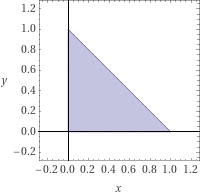
\includegraphics[scale=1]{1-1region.png}
    % \end{center}
    \begin{figure}[h]
    \centering        
        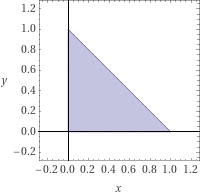
\includegraphics[scale=1]{1-1region.png}
        \caption{The joint density function $f(x,y)$ is nonzero in the shaded region.}
    \end{figure}
    As $x$ ranges from 0 to 1, $y$ ranges from 0 to $1-x$.
    To see this, draw a vertical slice upwards from any point on the $x$-axis until it intersects the line $x+y=1$.
    Our integral then becomes
    \begin{align*}
        k\int_0^1\int_0^{1-x}xy\ dydx &= k\int_0^1x\left[\frac{1}{2}y^2\right]_{y=0}^{1-x}dx\\
        &= \frac{k}{2}\int_0^1x(1-x)^2\ dx\\
        &= \frac{k}{2}\left[\frac{1}{4}x^4-\frac{2}{3}x^3 + \frac{1}{2}x^2\right]_{x=0}^{x=1}\\
        &= k/24.
    \end{align*}
    Since this expression must be equal to 1, we have $k=24$.

    Now let's compute the marginal pdf's of $X$ and $Y$.
    To get the marginal for $X$, we ``integrate out the $y$.''
    For any fixed $x$, the value of $y$ ranges between 0 and $1-x$, so we have
    \[
        f_X(x) = \int_{\R}f(x,y)\ dy = \int_0^{1-x}kxy\ dy = \frac{k}{2}x(1-x)^2 = 12x(1-x)^2.
    \]
    Similarly, for any fixed $y$, the value of $x$ ranges between 0 and $1-y$.
    \[
        f_Y(y) = \int_{\R}f(x,y)\ dx = \int_0^{1-y}kxy\ dx = \frac{k}{2}y(1-y)^2 = 12y(1-y)^2.
    \]
\end{example}

\begin{example}
    The joint density function of $X$ and $Y$ is given by
    \[
        f(x,y) = \begin{cases}
            2e^{-x}e^{-2y},&\text{if }0<x<\infty, 0<y<\infty\\
            0,&\text{otherwise.}
        \end{cases}
    \]

    Let's compute $\Pr[X>1, Y<1]$.
    To compute the probability of \emph{any} event, we simply integrate the joint density function over that event.
    In this case we have
    \begin{align*}
        \Pr[X > 1, Y< 1] &= \int_0^1\int_1^\infty2e^{-x}e^{-2y}\ dxdy\\
        &= \int_0^12e^{-2y}\left[-e^{-x}\right]_{x=1}^{x=\infty}dy\\
        &= 2e^{-1}\int_0^1e^{-2y}dy\\
        &= e^{-1}(1-e^{-2}).
    \end{align*}
\end{example}

In the case of a single random variable, the density and distribution functions are related by differentiation.
That is, if $X$ has density function $f$ and distribution function $F$, then
\[
    f(x) = \frac{d}{dx}F(x).
\]
The multivariable analogue is what you would probably expect.
If $X$ and $Y$ are jointly continuous with density function $f(x,y)$ and distribution function $F(x,y)$, then we have by Fubini's theorem
\begin{equation}\label{derivative of distribution is density}
    f(x,y) = \frac{\partial^2}{\partial x \partial y}F(x,y) = \frac{\partial^2}{\partial y\partial x}F(x,y).
\end{equation}
We aren't going to angst over the proof here, but this technically only holds for the values of $(x,y)$ where the partial derivatives are defined and continuous.










\subsection{Independent Random Variables}
Remember that we said that two \emph{events} $A$ and $B$ are independent if
\[
    \Pr[A\cap B] = \Pr[A]\cdot \Pr[B].
\]
We can carry this definition over to random variables.
\begin{definition}
    Let $X$ and $Y$ be random variables.
    Then $X$ and $Y$ are \emph{independent} if for any measurable sets $A$ and $B$ we have
    \[
        \Pr[X\in A, Y\in B] = \Pr[X\in A]\cdot \Pr[Y\in B].
    \]
\end{definition}

Let's show that this definition plays nicely with the machinery we defined in the previous section.

\begin{proposition}
    The discrete random variables $X$ and $Y$, taking values in $\mathcal X$ and $\mathcal Y$, respectively, are independent if and only if
    \begin{equation}\label{discrete indep}
        p(x,y) = p_X(x)p_Y(y)
    \end{equation}
    for all $x\in \mathcal X$ and $y\in \mathcal Y$.
\end{proposition}
\begin{proof}
    First let's suppose that $X$ and $Y$ are independent.
    Then we can consider the singleton sets $\{x\}$ and $\{y\}$ for any $x\in \mathcal X$, $y\in \mathcal Y$.
    \[
        p(x,y) = \Pr[X = x, Y=y] = \Pr[X=x]\Pr[Y=y] = p_X(x)p_Y(y).
    \]

    Now suppose that equation (\ref{discrete indep}) holds.
    Then for any sets $A\subseteq \mathcal X$ and $B\subseteq \mathcal Y$ we have
    \begin{align*}
        \Pr[X\in A, Y\in B] &= \sum_{x\in A, y\in B}p(x,y)\\
        &= \sum_{x\in A}p_X(x)\sum_{y\in B}p_Y(y)\\
        &= \Pr[X\in A]\Pr[Y\in B],
    \end{align*}
    so $X$ and $Y$ are independent.
\end{proof}


\begin{example}
    Suppose we perform $n+m$ independent trials, each having common success probability $p$.
    Let $X$ be the number of successes in the first $n$ trials and let $Y$ be the number of successes in the next $m$ trials.
    Are $X$ and $Y$ independent?
    Intuitively, knowing what happens in the first $n$ trials shouldn't tell us anything about what happens in the next $m$ trials, so we hope that $X$ and $Y$ are independent.
    Indeed, we have
    \[
        \Pr[X = x, Y=y] = \binom{n}{x}p^x(1-p)^{n-x}\binom{m}{y}p^y(1-p)^{m-y}= \Pr[X=x]\Pr[Y=y].
    \]

    Let's define a new random variable $Z$ to be the total number of successes in all $m+n$ trials.
    Are $X$ and $Z$ independent?
    Well if we know there are some successes in the first $n$ trials, then we definitely know that there are at least that many successes in total, so we suspect that these aren't independent.
    We have
    \begin{align*}
        p(x,z) &= \Pr[x\text{ successes in the first $n$ trials, $z$ successes total}]\\
        &= \Pr[x\text{ successes in the first $n$ trials, $z-x$ successes in the next $m$ trials}]\\
        &= \binom{n}{x}p^x(1-p)^{n-x}\binom{m}{z-x}p^{z-x}(1-p)^{m-z+x}.
    \end{align*}
    However,
    \begin{align*}
        p_X(x) &= \binom{n}{x}p^x(1-p)^{n-x}\\
        p_Z(z) &= \binom{n+m}{z}p^z(1-p)^{n+m-z}.
    \end{align*}
    It's easily seen that the product of these two quantities does not match up with the previous quantity, so $X$ and $Z$ are \emph{not} independent.
\end{example}

So we can check to see if two discrete random variables are independent by looking at their mass functions.
What about continuous random variables?
We should think of a discrete random variable's mass function as being analogous to a continuous random variable's density function, and this informs the next proposition.

\begin{proposition}
    If $X$ and $Y$ are continuous random variables, then they are independent if and only if
    \[
        f(x,y) = f_X(x)f_Y(y).
    \]
\end{proposition}
\begin{proof}
    Suppose $X$ and $Y$ are independent.
    This is really a statement about \emph{distribution} functions, not density functions, so we have
    \begin{equation}\label{continuous indep}
        \Pr[X\leq x, Y\leq y] = \Pr[X\leq x]\Pr[Y\leq y],
    \end{equation}
    which is equivalent to
    \[
        F(x,y) = F_X(x)F_Y(y).
    \]
    Now let's take the mixed $x$ and $y$ partial derivatives of both sides to obtain
    \[
        \frac{\partial^2}{\partial x\partial y}F(x,y) = \frac{\partial^2}{\partial x\partial y}\big(F_X(x)F_Y(y)\big) = \frac{\partial}{\partial x}F_X(x)\frac{\partial}{\partial y}F_Y(y).
    \]
    We arrived at the last equality using the fact that $F_X(x)$ is constant with respect to $y$ and $F_Y(y)$ is constant with respect to $x$.
    Since differentiation distributions gives us densities, we have
    \[
        f(x,y) = f_X(x)f_Y(y)
    \]
    as desired.

    Conversely, suppose that equation (\ref{continuous indep}) holds.
    We pretty much copy the proof of the previous proposition with integrals in place of sums.
    For any sets $A$ and $B$ we have
    \begin{align*}
        \Pr[X\in A, Y\in B] &= \int_A\int_Bf(x,y)\ dydx\\
        &= \int_Af_X(x)\ dx\int_Bf_Y(y)\ dy\\
        &= \Pr[X\in A]\Pr[Y\in B].
    \end{align*}
\end{proof}

So we have have independence if our joint density (or mass) function factors into the product of the marginals.
We can actually say more -- factoring into \emph{any} product of functions, each depending on just one variable, is enough.
\begin{proposition}
    Let $X$ and $Y$ be continuous random variables.
    Then $X$ and $Y$ are independent if and only if the joint density function can be factored as
    \begin{equation}\label{joint factors}
        f(x,y) = h(x)g(y)
    \end{equation}  
    for some functions $g$ and $h$.
\end{proposition}
\begin{proof}
    If $X$ and $Y$ are independent, then the previous proposition tells us that we can just take $g = f_X$ and $h = f_Y$.

    Conversely, suppose that $f(x,y) = h(x)g(y)$.
    Then
    \begin{align*}
        1 &= \int_\R\int_\R f(x,y)\ dxdy\\
        &= \int_\R h(x)\ dx\cdot \int_\R g(y)\ dy.
    \end{align*}
    But these last two integrals have to each be equal to some constants, $c_1$ and $c_2$, respectively.
    We also have
    \begin{align*}
        f_X(x) &= \int_\R f(x,y)\ dy\\
        &= \int_\R h(x)g(y)\ dy\\
        &= c_1 h(x).
    \end{align*}
    Similarly, $f_Y(y) = c_2g(y)$.
    Putting it all together, we have
    \begin{align*}
        f_X(x)f_Y(y) &= c_1h(x)\cdot c_2g(y)\\
        &= (c_1c_2)h(x)g(y)\\
        &= f(x,y).
    \end{align*}
\end{proof}

\begin{example}
Suppose $X$ and $Y$ are jointly continuous random variables with joint density
    \[
        f(x,y) = \begin{cases}
            kxy,&\text{if }(x,y)\in [0,1]^2\\
            0,&\text{otherwise.}
        \end{cases}
    \]
Are $X$ and $Y$ independent?
They'd definitely be independent it we could factor the joint density, but how does the piecewise nature of the density play into this?
Let's define the \emph{indicator function} for the set our density actually lives on.
That is, let $I(x,y)$ be defined by
\[
    I(x,y) = \begin{cases}
        1,&\text{if }(x,y)\in [0,1]^2\\
        0,&\text{otherwise.}
    \end{cases}
\]
That is, $I(x,y)$ indicates whether or not $(x,y)$ lives in the set $[0,1]^2$, the unit square in $\R^2$.
We go through the trouble of defining this function because we can use it to write our density as
\[
    f(x,y) = kxy\cdot I(x,y).
\]
The $kxy$ part is clearly a product of a function of only $x$ with a function of only $y$.
If we could factor the indicator function $I$ into functions of just $x$ and just $y$, then we will have shown independence.
Our ability to do this is going to come down to the nature of the set $[0,1]^2$.
Notice that $(x,y)\in [0,1]^2$ if and only if both coordinates live in $[0,1]$.
That is, if we define $\tilde{I}(x)$ by
\[
    \tilde{I}(x) = \begin{cases}
        1,&\text{if }x\in [0,1]\\
        0,&\text{otherwise,}
    \end{cases}
\]
then we have $I(x,y) = \tilde{I}(x)\tilde{I}(y)$, so our joint density factors as
\[
    f(x,y) = (kx\cdot \tilde{I}(x))(y\cdot \tilde{I}(y)),
\]
so $X$ and $Y$ are independent.
\end{example}

\begin{example}
Suppose $X$ and $Y$ are jointly continuous random variables with joint density
    \[
        f(x,y) = \begin{cases}
            kxy,&\text{if }x,y\geq 0, x+y\leq 1\\
            0,&\text{otherwise.}
        \end{cases}
    \]
Are $X$ and $Y$ independent?
This density looks a lot like the one from the previous exercise.
The difference here is that $f(x,y)$ behaves like $kxy$ on a different set this time.
Now $f$ lives on a triangle in the first quadrant rather than an axis-aligned square.
Proceeding in the same way as before, if we define
\[
    I(x,y) = \begin{cases}
        1,&\text{if }x,y\geq 0, x+y\leq 1\\
        0,&\text{otherwise,}
    \end{cases}
\]
Then we still have $f(x,y) = kxy\cdot I(x,y)$ like before.
Can we still factor it?
Well if we specify the $x$ coordinate to live between 0 and 1, then the $y$ coordinate needs to satisfy $0\leq y\leq 1-x$.
If we define the functions $I_1$ and $I_2$ by
\[
    I_1(x) = \begin{cases}
        1,&\text{if }x\in [0,1]\\
        0,&\text{otherwise,}
    \end{cases} \qquad
    I_2(x,y) = \begin{cases}
        1,&\text{if }0\leq y\leq 1-x\\
        0,&\text{otherwise,}
    \end{cases}
\]
then we do get the factorization
\[
    f(x,y) = kxy \cdot I_1(x)\cdot I_2(x,y),
\]
but this isn't helpful since $I_2(x,y)$ is a function of both $x$ and $y$.

This is \emph{not} a proof that $X$ and $Y$ aren't independent.
For all we know, there's some weird factorization of $f(x,y)$ we just haven't found yet.
Let's approach it a bit differently.
This is the same density from Example \ref{triangle density} and we found the marginal density functions to be
\[
    f_X(x) = \begin{cases}
        (k/2)x(1-x)^2,&\text{if }0\leq x \leq 1\\
        0,&\text{otherwise,}
    \end{cases}\qquad
    f_Y(y) = \begin{cases}
        (k/2)y(1-y)^2,&\text{if }0\leq y \leq 1\\
        0,&\text{otherwise.}
    \end{cases}
\]
Notice that we do \emph{not} have that $f(x,y) = f_X(x)f_Y(y)$ for all $x,y$ where these three functions are defined, so $X$ and $Y$ are \emph{not} independent.
\end{example}










\subsection{Sums of Independent Random Variables}
Say we have two real-valued random variables $X$ and $Y$.
We'll assume they're discrete for now.
Their sum $Z=X+Y$ is clearly a random variable as well.
How do the mass functions of $X$ and $Y$, $p_X$ and $p_Y$, and the joint mass function $p$ relate to the mass function of $X+Y$?
Well $p_Z(z) = \Pr[Z = z]$ and we can break the event $\{Z = z\}$ into the events
\[
    \{Z = z\} = \bigcup_{x}\{X = x, Y = z-x\}.
\]
To see this, note that in order for $X+Y = z$ to be true, $X$ can be anything so long as $Y = z-X$.
Moreover, these events are clearly disjoint since $X$ and $Y$ can only take one value at a time.
Since the probability of a \emph{disjoint} union is just the sum of the probabilities of the constituent events, we have
\[
    p_Z(z) = \sum_x \Pr[X = x, Y= z-x] = \sum_x p(x, z-x).
\]
Now if $X$ and $Y$ are independent, the joint density factors as $p(x,y) = p_X(x)p_Y(y)$ and we've proven the following proposition.
\begin{proposition}
    If $X$ and $Y$ are discrete random variables, then the probability mass function of $Z = X+Y$ is
    \[
        p_Z(z) = \sum_x p_X(x)p_Y(z-x).
    \]
\end{proposition}

\begin{example}
    Suppose $X$ and $Y$ are independent random variables, both taking values in $\{1, 2, \ldots, n\}$ uniformly at random (if $n=6$, then you can think $X$ and $Y$ as the outcomes of dice rolls).
    If we set $Z = X+Y$, then the previous proposition tells us that
    \[
        p_Z(z) = \sum_{j = 1}^np_X(j)p_Y(z-j).
    \]
    Now it might be tempting to just set $p_X(j)$ and $p_Y(z-j)$ to $1/n$.
    If this were the case, then we would have $p_Z(z) = 1/n$ for each $z$.
    But this definitely doesn't line up with our intuition -- when we roll two dice, some outcomes are more likely than others (there's only one way to roll a 2, but six ways to roll a 7).
    The problem is that $p_Y(z-j)$ isn't always $1/n$.
    Indeed, if $z-j < 1$, then $Y$ never takes the value $z-j$.

    We can fix this by looking at the conditions that make $p_X(j)$ and $p_Y(z-j)$ \emph{both} positive.
    In order for this to happen, we need $1\leq j\leq n$ \emph{and} $1\leq z-j\leq n$ to both hold.
    Isolating $j$ gives
    \[
        z-n \leq j\leq z-1 \qquad\text{and}\qquad 1\leq j\leq n.
    \]
    If $z$ is between $2$ and $n$ this becomes
    \[
        p_Z(z) = \sum_{j=1}^{z-1}p_X(j)p_Y(z-j) = \sum_{j=1}^{z-1}\frac{1}{n^2} = \frac{z-1}{n^2}. 
    \]
    On the other hand, if $z$ is between $n+1$ and $2n$ we have
    \[
        p_Z(z) = \sum_{j=z-n}^n p_X(j)p_Y(z-j) = \sum_{j=z-n}^n\frac{1}{n^2} = \frac{2n-z+1}{n^2}.
    \]
    So in total we have
    \[
        p_Z(z) = \begin{cases}
            (z-1)/n^2,&\text{if }2\leq z \leq n\\
            (2n-z+1)/n^2,&\text{if }n+1\leq z\leq 2n.
        \end{cases}
    \]
    Importantly, we have that the sum of two uniform random variables is \emph{not} another uniform random variable.
\end{example}

\begin{example}\label{sum of Poissons}
    If $X$ and $Y$ are independent Poisson random variables with respective parameters $\lambda_1$ and $\lambda_2$, let's compute the distribution of $X+Y$.

    We have that
    \begin{align*}
        \Pr[X+Y = n] &= \sum_{k=0}^n\Pr[X = k, Y = n-k]\\
        &= \sum_{k=0}^n\Pr[X=k]\Pr[Y=n-k]\\
        &= \sum_{n=0}^n e^{-\lambda_1}\frac{\lambda_1^k}{k!}e^{-\lambda_2}\frac{\lambda_2^{n-k}}{(n-k)!}\\
        &= e^{-(\lambda_1+\lambda_2)}\sum_{k=0}^n\frac{\lambda_1^k\lambda_2^{n-k}}{k!(n-k)!}.
    \end{align*}
    Now the sum at the end should remind us of the binomial theorem since it has a product of two terms whose powers sum to $n$.
    We almost have the correct binomial coefficient too.
    We just need to multiply and divide by $n!$.
    \begin{align*}
        \Pr[X+Y = n] &= e^{-(\lambda_1+\lambda_2)}\sum_{k=0}^n\frac{\lambda_1^k\lambda_2^{n-k}}{k!(n-k)!}\\
        &= \frac{e^{-(\lambda_1+\lambda_2)}}{n!} \sum_{k=0}^n\frac{n!}{k!(n-k)!}\lambda_1^k\lambda_2^{n-k}\\
        &= \frac{e^{-(\lambda_1+\lambda_2)}}{n!}(\lambda_1+\lambda_2)^n.
    \end{align*}
    This is the mass function of a Poisson random variable with parameter $\lambda_1+\lambda_2$.
\end{example}

Let's look at the case of continuous random variables.
The analogy (mass functions $\iff$ densities) and (sums $\iff$ integrals) leads us to the following proposition.
\begin{proposition}
    Suppose $X$ and $Y$ are jointly continuous real-valued random variables with joint density function $f$.
    Then the variable $Z = X+Y$ has density function
    \[
        f_Z(z) = \int_\R f(x, z-x)\ dx = \int_\R f(z-y, y)\ dy.
    \]
    In particular, if $X$ and $Y$ are independent, then this becomes
    \[
        f_Z(z) = \int_\R f_X(x)f_Y(z-x)\ dx = \int_\R f_X(z-y)f_Y(y)\ dy.
    \]
\end{proposition}
\begin{proof}
    Let's look at the distribution function for $Z$.
    That is, for any real $a$ we have
    \[
        F_Z(a) = \Pr[Z\leq a] = \Pr[X+Y \leq a] = \int_{x + y\leq a}f(x,y)\ dxdy.
    \]
    Upon looking at a diagram of this region, we turn this into an iterated integral.
    \[
        F_Z(a) = \int_\R \int_{-\infty}^{a-x}f(x, y)\ dxdy.
    \]
    Now if we do the substitution $y = z-x$, this becomes
    \[
        F_Z(a) = \int_\R\int_{-\infty}^af(x, z-x)\ dzdx = \int_{-\infty}^a\int_{-\infty}^\infty f(x, z-x)\ dxdz.
    \]
    We used Fubini's theorem to switch the order of integration at the end.
    Now we can use the fundamental theorem of calculus to take the derivative of both sides with respect to $a$ to get the probability density function of $Z$,
    \[
        f_Z(z) = \int_\R f(x, z-x)\ dx.
    \]
    Now if $X$ and $Y$ are independent, we can factor the joint density function to get $f(x,z-x) = f_X(x)f_Y(z-x)$.
\end{proof}

\begin{example}
    Let's do the continuous version of the previous example.
    That is, suppose $X$ and $Y$ are independent random variables taking values in the interval $[0, 1]$ uniformly.
    By the above proposition, the density of $Z= X+Y$ is given by
    \[
        f_Z(z) = \int_\R f_X(x)f_Y(z-x)\ dx.
    \]
    To actually compute this integral, we need to know the values of $x$ that make $f_X(x)$ and $f_Y(z-x)$ positive.
    Since the density of the uniform distribution is given by
    \[
        f_X(x) = \begin{cases}
            1,&\text{if }x\in [0,1]\\
            0,&\text{otherwise,}
        \end{cases}
    \]
    we have that $f_X(x)$ is positive if and only if $0\leq x\leq 1$ and $f_Y(z-x)$ is positive if and only if $0\leq z-x\leq 1$.
    When we combine these, we see that the values of $x$ that make both inequalities true depend on what $z$ is.
    In particular, when $0\leq z\leq 1$, we need $0\leq x \leq z$, and when $1\leq z\leq 2$, we need $z\leq x\leq 1$.
    So if $0\leq z\leq 1$, we have
    \[
        f_Z(z) = \int_0^z 1\ dz = z
    \]
    and when $1\leq z\leq 2$ we have
    \[
        f_Z(z) = \int_z^1 1\ dz = 1-z.
    \]
\end{example}

\begin{example}
    Let $X$ and $Y$ be independent standard normal random variables (that is, they both have mean 0 and variance 1).
    Recall that the density of $X$ is then
    \[
        f_X(x) = \frac{1}{\sqrt{2\pi}}e^{-x^2/2}.
    \]
    Let's compute the density of the sum $Z = X+Y$.
    We have
    \begin{align*}
        f_Z(z) &= \int_\R f_X(x)f_Y(z-x)\ dx\\
        &= \int_\R \frac{1}{\sqrt{2\pi}}e^{-x^2/2}\cdot \frac{1}{\sqrt{2\pi}}e^{-(z-x)^2/2}\ dx\\
        &= \frac{1}{2\pi}\int_\R e^{-x^2 + zx - z^2/2}\ dx.
    \end{align*}
    At this point, we complete the square in the exponent.
    \[
        -x^2 + zx - z^2/2 = -x^2 + zx -z^2/4 + z^2/4 - z^2/2 = -(x-z/2)^2 - z^2/4.
    \]
    So the density becomes
    \begin{align*}
        f_Z(z) &= \frac{1}{2\pi}e^{-z^2/4}\int_\R e^{-(x-z/2)^2}dx = \frac{1}{\sqrt{2\pi}\cdot \sqrt{2}}e^{-z^2/4}.
    \end{align*}
    Here we've used the fact that $\int_\R e^{-x^2}\ dx = \sqrt{\pi}$ along with a simple substitution.
    \textcolor{red}{In class, I mistakenly said this integral was $\sqrt{2\pi}$.}
    Note that this is the density of a normal random variable having mean 0 and variance 2.
\end{example}

So the sum of two independent standard normal random variables is again a normal random variable.
More generally, the sum of arbitrarily many independent normal random variables is again a normal random variable.
The proof of this more general fact is pretty much the same, but the algebra is a little messier.

\begin{theorem}
    If $X_1, X_2, \ldots, X_n$ are independent normal random variables with mean $\mu_i$ and variance $\sigma_i^2$, respectively, then the sum $\sum_{i=1}^nX_i$ is normally distributed with mean $\sum_{i=1}^n\mu_i$ and variance $\sum_{i=1}^n\sigma_i^2$.
\end{theorem}


\begin{example}
    The number of candies in a standard bag of plain M\&M's is normally distributed with a mean of 55 candies and a standard deviation of 2 candies.
    The number of candies in a sharing size bag of plain M\&M's is also normally distributed with a mean of 340 candies and a standard deviation of 3 candies.
    What is the probability that six standard bags of M\&M's together contain more candies than one sharing bag?

    Let $X_1, \ldots, X_6$ be the number of candies in the six standard bags and let $Y$ be the number of candies in the sharing sized bag.
    Then we want the probability that $X_1 + \cdots + X_6 - Y > 0$.
    By the above theorem, this sum is a normal random variable with mean $6\cdot 55 - 340 = -10$ candies and variance $6\cdot 2 + 3 = 15$.

    We can compute the desired probability by using a $z$-table as follows.
    If we let $W = X_1 + \cdots + X_6 - Y$, then
    \[
        \Pr[W > 0] = \Pr\left[\frac{W-(-10)}{\sqrt{15}} > \frac{0 - (-10)}{\sqrt{15}}\right].
    \]
    Now $Z = (W+10)/\sqrt{15}$ is a standard normal random variable, and a $z$-table lets us look up the probability that such a random variable is less that $t$ for many values of $t$.
    Using table 5.1 in the textbook, we see that $\Pr[Z < 10/\sqrt{15}] \approx \Pr[Z< 2.58] \approx  .9951$.
    Thus,
    \[
        \Pr[Z > 2.58] \approx 1- .9951 = .0049.
    \]
\end{example}










\subsection{Conditional Distributions -- Discrete Random Variables}

Let's briefly recall the basics of conditional probability.
If $E$ and $F$ are events, then $\Pr[E \mid F]$ (read ``the probability of $E$ given $F$'') is defined to be
\[
    \Pr[E\mid F] = \frac{\Pr[E \cap F]}{\Pr[F]}.
\]
Intuitively, $\Pr[E\mid F]$ is the probability that $E$ happens with the additional information that $F$ happened.
The above definition quantitatively captures this idea when you think of it as shrinking your probability space to just $F$.
If the events $E$ and $F$ are independent, then we  have
\[
    \Pr[E\mid F] = \frac{\Pr[E\cap F]}{\Pr[F]} = \frac{\Pr[E]\cdot \Pr[F]}{\Pr[F]} = \Pr[E].
\]
Intuitively this makes sense -- if $E$ and $F$ are independent, then learning that $E$ happened shouldn't tell you anything about whether or not $F$ happened.
Quantitatively, this means that $E\cap F$ makes up the same fraction of $F$ as $E$ does in the original probability space.

Now let's think about conditional probability in the context of random variables.
\begin{definition}
    Let $X$ and $Y$ be discrete random variables.
    Then the \emph{conditional probability mass function of $X$, given that $Y = y$} is
    \[
        p_{X\mid Y}(x\mid y) = \Pr[X = x\mid Y = y] = \frac{p(x,y)}{p_Y(y)}.
    \]
\end{definition}

This definition corresponds to plugging the events $\{X = x\}$ and $\{Y = y\}$ into the definition of conditional probability.

\begin{example}
    Say 100 people are asked for their handedness (right-handed or left-handed) and sex (male or female). The survey produces the following table.
    \begin{center}
    \begin{tabular}{|c || c | c|}
        \hline
           & L & R\\
        \hline
         M & 4 & 44\\
         F & 9 & 43\\
         \hline
    \end{tabular}
    \end{center}
    Select a person from this population at random and let $X$ be their handedness and $Y$ be their sex.
    Let's find the conditional pmf of $X$ given that we selected a female.
    \begin{align*}
        p_{X\mid Y}(L \mid F) &= \frac{\frac{9}{100}}{\frac{9}{100} + \frac{43}{100}} = \frac{9}{52}\\
        p_{X\mid Y}(R\mid F) &= \frac{\frac{43}{100}}{\frac{9}{100} + \frac{43}{100}} = \frac{43}{52}.
    \end{align*}
\end{example}

\begin{example}
    Suppose $X$ and $Y$ are independent Poisson random variables with respective parameters $\lambda_1$ and $\lambda_2$.
    Let's find the conditional distribution of $X$ given that $X+Y = n$.

    It's important to note that just because $X$ and $Y$ are independent, it does not follow that $X$ and $X+Y$ are independent.
    Indeed, if we know that $X = n$, then $X+Y$ must be at least $n$.
    Now we have that
    \begin{align*}
        \Pr[X = k\mid X+Y = n] &= \frac{\Pr[X=k, X+Y = n]}{\Pr[X+Y = n]}\\
        &= \frac{\Pr[X=k, Y = n-k]}{\Pr[X+Y=n]}\\
        &= \frac{\Pr[X=k]\cdot \Pr[Y = n-k]}{\Pr[X+Y=n]}.
    \end{align*}
    Now it looks like we need to know the distribution of the sum $X+Y$.
    We figured this out in Example \ref{sum of Poissons} where we saw what $X+Y\sim Pois(\lambda_1+\lambda_2)$, so we have
    \begin{align*}
        \Pr[X=k\mid X+Y = n] &= \frac{e^{-\lambda_1}\lambda_1^k}{k!}\cdot \frac{e^{-\lambda_2}\lambda_2^{n-k}}{(n-k)!} \cdot \frac{n!}{e^{-(\lambda_1+\lambda_2)}(\lambda_1+\lambda_2)^n}\\
        &= \binom{n}{k}\left(\frac{\lambda_1}{\lambda_1+\lambda_2}\right)^k\left(\frac{\lambda_2}{\lambda_1+\lambda_2}\right)^{n-k}.
    \end{align*}
    This is a binomial distribution with $n$ trials and success probability $\lambda_1/(\lambda_1+\lambda_2)$.
\end{example}

If $X$ and $Y$ are discrete random variables, we can condition on a particular outcome $Y = y$ to obtain a new random variable.
That is, the random variable $(X\mid Y = y)$ is itself a random variable.
In particular, we can compute its expected value.

\[
    E[X\mid Y=y] = \sum_x x\cdot p_{X\mid Y}(x\mid y).
\]

% \begin{example}
%     You have two identical envelopes in front of you.
%     One contains twice as much money as the other.
%     You are asked to choose one of the envelopes for yourself.
%     You pick one at random, open it, and observe its contents.
%     Then you have the choice to switch your envelope for the other one.
%     What should you do?

%     Let's go for a strategy that maximizes our \emph{expected} payoff.
%     Why this is the right thing to do is probably intuitive, but we'll hopefully go into this in more detail at another time.
%     Let $X$ be the amount of money in the envelop you \emph{didn't} pick and let $Y$ be the amount of money in the envelope you opened.
%     Since you had a 1/2 chance of picking the envelope with the larger amount, we have
%     \[
%         (X \mid Y=y) = \begin{cases}
%             2y,&\text{with probability }1/2\\
%             y/2,&\text{with probability }1/2.
%         \end{cases}
%     \]
%     Let's compute the expectation.
%     \begin{align*}
%         E[X\mid Y=y] &= 2y\cdot \frac{1}{2} + \frac{y}{2}\cdot \frac{1}{2}\\
%         &= y + \frac{y}{4}\\
%         &= \frac{5}{4}y.
%     \end{align*}
%     In other words, regardless of what you saw in the first envelope, we expect to see 25\% more money in the other envelope, so we should always switch envelopes according to this strategy.
% \end{example}










\subsection{Conditional Distributions -- Continuous Random Variables}
Using the mass function $\iff$ density function analogy, we arrive at the following definition.

\begin{definition}
    Let $X$ and $Y$ be continuous random variables with joint probability density function $f$.
    Then the \emph{conditional probability density function of $X$ given that $Y=y$ is}
    \[
        f_{X\mid Y}(x\mid y) = \frac{f(x,y)}{f_Y(y)}.
    \]
    Of course, this only makes sense for the values of $y$ where $f_Y(y)>0$.
\end{definition}

To see why this definition is ``correct,'' remember that $f_X(x)\ dx$ is roughly the probability that $X$ lies between $x$ and $x+dx$.
In particular,
\begin{align*}
    f_{X\mid Y}(x\mid y)\ dx &= \frac{f(x,y)\ dxdy}{f_Y(y)\ dy}\\
    &\approx \frac{\Pr[x \leq X\leq x+dx, y\leq Y \leq y+dy]}{\Pr[y\leq Y\leq y+dy]}\\
    &= \Pr[x\leq X \leq x+dx \mid y\leq Y \leq y+dy].
\end{align*}

Just as in the case of discrete random variables, we can condition $X$ on $Y=y$ and take the expectation.
\[
    E[X\mid Y=y] = \int_\R xf_{X\mid Y}(x\mid y)\ dx.
\]

\begin{remark}
    If $X$ and $Y$ are independent continuous random variables, then
    \[
        f_{X|Y}(x\mid y) = \frac{f(x,y)}{f_Y(y)} = \frac{f_X(x)f_Y(y)}{f_Y(y)} = f_X(x)
    \]
    and
    \[
        E[X\mid Y=y] = \int_\R x f_{X\mid Y}(x\mid y)\ dx = \int_\R x f_X(x)\ dx = E[X].
    \]
    That is, if $X$ and $Y$ are independent, conditioning $X$ on the event $Y=y$ ``doesn't do anything.''
\end{remark}

\begin{example}
    The joint density of $X$ and $Y$ is given by
    \[
        f(x,y) = \frac{12}{5}x(2-x-y)\qquad (x,y)\in [0,1]^2.
    \]
    Let's compute the conditional density of $X$ given that $Y=y$ then compute $E[X\mid Y=1/3]$.

    Since $f_{X\mid Y}(x\mid y) = f(x,y)/f_Y(y)$, it looks like we need to find the marginal density function $f_Y(y)$.
    We can find this by ``integrating out the $x$''.
    \begin{align*}
        f_Y(y) &= \int_0^1 f(x,y)\ dx\\
        &= \int_0^1 \frac{12}{5} x(2-x-y)\ dx\\
        &= \cdots\\
        &= \frac{12}{5}\left(\frac{2}{3} - \frac{y}{2}\right).
    \end{align*}
    So we have 
    \[
        f_{X\mid Y}(x\mid y) = \frac{x (2-x-y)}{\frac{2}{3} - \frac{y}{2}} = \frac{6x(2-x-y)}{4-3y}
    \]
    for any $x, y\in [0,1]^2$.

    Now for the conditional expectation.
    \begin{align*}
        E[X\mid Y=1/3] &= \int_0^1 xf_{X\mid Y}(x\mid 1/3)\ dx\\
        &= \int_0^1 \frac{6x^2(\frac{5}{3}-x)}{3}\ dx\\
        &= \cdots\\
        &= \frac{11}{10}.
    \end{align*}
\end{example}


\begin{example}
    A particle with mass 1 splits into a smaller particle and some energy, where the mass of the smaller particle is a uniform $[0,1]$ random variable.
    The smaller particle then splits in the same way.
    What is the distribution of the mass of the final particle?

    Let $Y$ be the mass of the particle after the first split and let $X$ be the mass of the final particle.
    Then $Y\sim unif(0,1)$ and $(X\mid Y = y) \sim unif(0, y)$.
    So we know these density functions
    \[
        f_Y(y) = 1\quad\text{if }y\in [0,1],\qquad f_{X\mid Y}(x\mid y) = \frac{1}{y}\quad\text{if }x\in [0,y].
    \]
    Since we know the conditional and marginal densities, we can reconstruct the joint density.
    \[
        f(x,y) = f_Y(y)\cdot f_{X|Y}(x\mid y) = \frac{1}{y}\quad\text{if }0\leq x \leq y,\ 0\leq x\leq y.
    \]
    Now we can get the density of $x$ by ``integrating out the $y$.''
    \[
        f_X(x) = \int_x^1\frac{1}{y}\ dy = -\ln x\quad \text{for }x\in (0,1].
    \]
\end{example}


\begin{example}
    The lifetime of a light bulb has conditional distribution $Exp(\Lambda)$, where $\Lambda \sim unif(a,b)$ (maybe the fuse in the bulb is randomly selected).
    Find the marginal distribution of the lifetime of the light bulb.

    We're given the following densities
    \[
        f_{X\mid \Lambda}(x\mid \lambda) = \lambda e^{-\lambda x}\quad\text{if } x\geq 0\qquad f_\Lambda(\lambda) = \frac{1}{b-a}\quad\text{if } a\leq \lambda \leq b.
    \]
    We want the density $f_X(x)$.
    Like in the previous example, we use the marginal and conditional densities to reconstruct the joint density.
    \[
        f_{X, \Lambda}(x, \lambda) = f_\Lambda(\lambda)f_{X\mid \Lambda}(x\mid \lambda) = \frac{1}{b-a}\lambda e^{-\lambda x}\quad\text{if }a\leq \lambda \leq b,\ x\geq 0.
    \]
    Now we can find the density of $X$ by integrating out the $\lambda$.
    \begin{align*}
        f_X(x) &= \int_a^b \frac{\lambda e^{-\lambda x}}{b-a}\ d\lambda\\
        &= \cdots\\
        &= \frac{e^{-ax}(1+ax) - e^{-bx}(1+bx)}{x^2(b-a)},
    \end{align*}
    for any $x\geq 0$.
\end{example}










\subsection{Joint Probability Distribution of Functions of Random Variables}

Suppose $X\sim \Unif [0,1]$.
What is the distribution of $Y = X^2?$
The range of $Y$ is still $[0,1]$, but we shouldn't expect $Y$ to be a uniform random variable -- ``most'' numbers in $[0,1]$ have small squares.
We can directly compute the distribution function.
\begin{align*}
    F_Y(t) &= \Pr[Y\leq t]\\
    &= \Pr[X^2 \leq t]\\
    &= \Pr[X \leq \sqrt{t}]\\
    &= \sqrt{t}.
\end{align*}
Differentiating both sides gives the density of $Y$, $f_Y(t) = \frac{1}{2\sqrt{t}}$.
In total, we inverted the function $y = x^2$ and then took a derivative.
\begin{proposition}
    Let $X$ be a continuous random variable and let $Y = g(X)$ for some continuously differentiable function $g$.
    Then the density of $Y$ is given by
    \[
        f_Y(y) = \frac{f(x)}{|dg/dx|},
    \]
    where $x = g^{-1}(y)$.
    (Technically, this holds for $x$ such that $|dg/dx|$ is nonzero)
\end{proposition}
\begin{proof}
    We repeat the previous example, just in more generality.
    Start by computing the distribution function.
    \begin{align*}
        F_Y(y) &= \Pr[Y\leq y]\\
        &= \Pr[g(X)\leq y]\\
        &= \Pr[X \leq g^{-1}(y)]\\
        &= F_X(g^{-1}(y)).
    \end{align*}
    Now we differentiate both sides, recalling that $[g^{-1}(y)]' = 1/g'(x)$ and $x = g^{-1}(y)$.
    \[
        f_Y(y) = \frac{f_X(g^{-1}(y))}{g'(x)} = \frac{f_X(x)}{|dg/dx|}.
    \]
\end{proof}


\begin{example}
    Suppose $X\sim \mathcal{N}(0, 1)$.
    Let's find the density function of $Y = X^2$.
    In terms of the above proposition, $g(x) = x^2$ and we have
    \[
        f_Y(y) = \frac{f_X(x)}{g'(x)} = \frac{1}{2x}\cdot \frac{1}{\sqrt{2\pi}}e^{-x^2/2}.
    \]
    Now we should get the right-hand side in terms of $y$.
    Since $y = x^2$ here, $x = \sqrt{y}$ and we have
    \[
        f_Y(y) = \frac{1}{2\sqrt{2\pi y}}e^{-y/2}.
    \]
    For those familiar with statistics, $Y$ is a $\chi^2$ random variable with one degree of freedom.
\end{example}

The multivariable version of the above proposition is spiritually the same and has pretty much the same proof.
\begin{theorem}\label{change of variables}
    Suppose $X_1$ and $X_2$ are continuous random variables with joint density function $f_{X_1, X_2}$.
    Then if $g_1$ and $g_2$ are continuously differentiable functions $\R^2\to \R$, and
    \[
        Y_1 = g_1(X_1, X_2)\qquad\text{and}\qquad Y_2 = g_2(X_1, X_2),
    \]
    then the joint density of $Y_1$ and $Y_2$ is given by
    \[
        f_{Y_1, Y_2}(y_1, y_2) = f_{X_1, X_2}(x_1, x_2)|J(x_1, x_2)|^{-1},
    \]
    where $J$ is the Jacobian determinant,
    \[
        J(x_1, x_2) = \det \begin{bmatrix}
            \partial g_1/\partial x_1 & \partial g_1/\partial x_2\\
            \partial g_2/\partial x_1 & \partial g_2/\partial x_2
        \end{bmatrix}.
    \]
\end{theorem}

\begin{example}
    Suppose $X_1$ and $X_2$ are independent exponential random variables with parameter $\lambda = 1$.
    Let $Y_1 = X_1 + X_2$ and $Y_2 = X_1 - X_2$.
    Let's find the joint density function of $Y_1$ and $Y_2$.

    In the context of Theorem \ref{change of variables}, $g_1(x_1, x_2) = x_1+x_2$ and $g_2(x_1, x_2) = x_1 - x_2$.
    Our Jacobian determinant is
    \[
        J(x_1, x_2) = \det \begin{bmatrix}
            1 & 1\\
            1 & -1
        \end{bmatrix} = -2.
    \]
    Consequently,
    \[
        f_{Y_1, Y_2}(y_1, y_2) = f_{X_1, X_2}(x_1, x_2)|J(x_1, x_2)|^{-1} = f_{X_1}(x_1)f_{X_2}(x_2)\cdot \frac{1}{2} = \frac{e^{-x_1-x_2}}{2} = \frac{e^{-y_1}}{2}.
    \]
    We used the independence of $X_1$ and $X_2$ to split the joint density of $X_1$ and $X_2$.
    Now what values of $y_1$ and $y_2$ does this hold for?
    To do this, we find $x_1$ and $x_2$ in terms of $y_1$ and $y_2$.
    We can easily check that
    \[
        x_1 = \frac{y_1+y_2}{2}\qquad\text{and}\qquad x_2 = \frac{y_1-y_2}{2}.
    \]
    Since $0\leq x_1\leq 1$ and $0\leq x_2\leq 1$, we have
    \[
        0 \leq y_1+y_2 \leq 2\qquad\text{and}\qquad 0\leq y_1-y_2\leq 2.
    \]

    How would we find the marginal density functions of $Y_1$ and $Y_2$?
\end{example}


\begin{example}
    Suppose we pick a random point $(X,Y)$ in the plane by choosing its coordinates one at a time, independently from a standard normal distribution.
    Let's find the distribution of the point's polar coordinates.

    Remember that the polar coordinates of $(X, Y)$ are
    \[
        R = \sqrt{X^2+Y^2},\qquad \Theta = \arctan (Y/X),
    \]
    when $X$ and $Y$ are both positive (we need to change $\Theta$ when we're in the other quadrants).
    In the context of Theorem \ref{change of variables}, we'll let $g_1(x,y) = \sqrt{x^2+y^2}$ and $g_2(x,y) = \arctan (y/x)$.
    Our Jacobian determinant is then
    \[
        J(x,y) = \det \begin{bmatrix}
            x/\sqrt{x^2+y^2} & y/\sqrt{x^2+y^2}\\
            -y/(x^2+y^2) & x/(x^2+y^2)
        \end{bmatrix} = 1/\sqrt{x^2+y^2}.
    \]
    Now the conditional joint density of $X$ and $Y$, \emph{given that $X$ and $Y$ are both positive}, is
    \[
        f(x,y\mid X>0, Y>0) = \frac{f(x,y)}{\Pr[X>0, Y>0]} = \frac{f(x,y)}{4} = \frac{2}{\pi}e^{-(x^2+y^2)/2},
    \]
    provided that $x,y>0$.
    By our theorem, the conditional joint density of $R$ and $\Theta$, given that $X$ and $Y$ are both positive, is
    \[
        f_{R, \Theta}(r, \theta\mid X>0, Y>0) = f(x,y\mid X>0, Y>0)|J(x,y)|^{-1} = \frac{2}{\pi}\sqrt{x^2+y^2}e^{-(x^2+y^2)/2}.
    \]
    In terms of $r$ and $\theta$, this becomes
    \[
        f_{R, \Theta}(r, \theta\mid X>0, Y>0) = \frac{2}{\pi}re^{-r^2/2},
    \]
    provided that $x$ and $y$ are both positive, i.e., that $r>0$ and $0\leq \theta \leq \pi/2$.

    The exact same argument gives us the conditional distributions for the other possible values of $X$ and $Y$.
    The only difference is that in each quadrant, we have to slightly modify our expression for $\theta$.
    For example, in quadrant II where $x<0$ and $y>0$, $\theta = \pi- \arctan (y/x)$.
    Importantly, this doesn't change the value of $|J(x,y)|$.
    In total, we have
    \begin{align*}
        f_{R, \Theta}(r, \theta\mid X<0, Y>0) &= \frac{2}{\pi}re^{-r^2/2}\\
        f_{R, \Theta}(r, \theta\mid X<0, Y<0) &= \frac{2}{\pi}re^{-r^2/2}\\
        f_{R, \Theta}(r, \theta\mid X>0, Y<0) &= \frac{2}{\pi}re^{-r^2/2}.
    \end{align*}
    Putting it all together, we see that
    \[
        f_{R, \Theta}(r,\theta) = \frac{1}{2\pi}re^{-r^2/2},\quad 0<\theta<2\pi,\ 0<r<\infty.
    \]

    In particular, since the joint density of $R$ and $\Theta$ factors into a product of functions, one depending on $r$ and the other on $\theta$ (really, there is no function of $\theta$ since the density doesn't depend on $\theta$ at all), we see that $R$ and $\Theta$ are independent!
\end{example}

\begin{example}
    Suppose we really want to sample from a standard normal distribution, but we only know how to generate uniform $[0,1]$ random variables.
    We'll use the previous example as our starting point.
    If we could somehow generate the variables $R$ and $\Theta$ (as in the previous example), then since
    \[
        X = R\cos \Theta\qquad\text{and}\qquad Y = R\sin \Theta,
    \]
    we could generate $X$ and $Y$, which are independent standard normal random variables.
    It's definitely easy to generate $\Theta$, since this variable is $\Unif (0, 2\pi)$.
    Unfortunately, it's not super clear how to generate $R$.

    If, in the previous example, we instead looked for the joint density of $R^2 = X^2+Y^2$ and $\Theta = \arctan (Y/X)$ (assuming for now that $X, Y\geq 0$), then we should take $d = g_1(x, y) = x^2+y^2$ and $\theta = g_2(x,y) = \arctan (y/x)$ in Theorem \ref{change of variables}.
    In this case, our Jacobian becomes.
    \[
        J(x,y) = \det \begin{bmatrix}
            2x & 2y\\
            -y/(x^2+y^2) & x/(x^2+y^2)
        \end{bmatrix} = 2.
    \]
    Following the same procedure as before, we get the joint density
    \[
        f_{R^2, \Theta}(d, \theta) = f(x,y)|J(x,y)|^{-1} = \frac{1}{2}e^{-d/2}\cdot \frac{1}{2\pi}.
    \]
    In particular, $R^2$ and $\Theta$ are independent and $R^2$ is an exponential random variable with parameter $1/2$.

    Now we claim that we can easily generate $R^2$.
    Suppose $U_1$ is a $\Unif [0,1]$ random variable and consider the quantity $-2\ln U_1$.
    Since $U_1$ is a $\Unif [0,1]$ variable, its distribution function is $F_{U_1}(u_1) = u_1$ and we have
    \begin{align*}
        \Pr[-2\ln U_1 \leq u_1] &= \Pr[U_1 \geq e^{-u_1/2}]\\
        &= 1-e^{-u_1/2}.
    \end{align*}
    If we differentiate both sides with respect to $u_1$, we see that the density of $-2 \ln U_1$ is $\frac{1}{2}e^{-U_1/2}$, so it's an exponential random variable with parameter $1/2$ -- just like $R^2$.
    Putting it all together, if $U_2$ is a $\Unif [0,1]$ random variable independent from $U_1$, then
    \[
        X = \sqrt{-2 \ln U_1} \cos (2\pi U_2),\qquad Y = \sqrt{-2 \ln U_1}\sin(2\pi U_2)
    \]
    are independent standard normal random variables.
\end{example}










\section{Properties of Expectation}
\subsection{Introduction}
Recall the definitions of expected value.
\begin{definition}
    If $X$ is a discrete real-valued random variable with probability mass function $p$, then its expected value (also called its expectation) is defined to be
    \[
        E[X] = \sum_x x p(x).
    \]
    If $X$ is a continuous random variable with density $f$, then its expected value is defined to be
    \[
        E[X] = \int_\R x f(x)\ dx.
    \]
\end{definition}

One basic fact is that if the (discrete) variable $X$ takes values between $a$ and $b$ with probability 1, then
\begin{align*}
    E[X] &= \sum_{x: p(x)>0}x p(x)\\
    &\geq \sum_{x: p(x) > 0} ap(x)\\
    &= a\sum_{x: p(x)>0}p(x)\\
    &= a.
\end{align*}
The same idea shows that $E[X]<b$ and the same argument applies to continuous random variables.










\subsection{Expectation of Sums of Random Variables}

Let's recall a couple of basic facts about expectation and then generalize them to multiple random variables.

\begin{lemma}\label{prob integral}
    If $X$ is a continuous random variable, then
    \[
        E[X]= \int_0^\infty \Pr[X > t]\ dt - \int_{-\infty}^0 \Pr[X< t]\ dt.
    \]
\end{lemma}
\begin{proof}
    If we assume that $X$ has density $f$, then we just change the order of integration (this is called Fubini's theorem).
    \begin{align*}
        \int_0^\infty \Pr[X > t]\ dt - \int_{-\infty}^0 \Pr[X<t]\ dt &= \int_0^\infty \int_t^\infty f(x)\ dxdt - \int_{-\infty}^0 \int_{-\infty}^t f(x)\ dxdt\\
        &= \int_0^\infty f(x)\int_0^xdtdx - \int_{-\infty}^0f(x)\int_x^0dtdx\\
        &= \int_0^\infty xf(x)\ dx - \int_{-\infty}^0 (-x)f(x)\ dx\\
        &= E[X].
    \end{align*}
\end{proof}

Using this lemma, we can prove the following obvious-looking theorem.

\begin{theorem}\label{LOTUS 1var}
    If $X$ is a continuous random variable with density $f$ and $g:\R\to \R$ is a continuous function, then
    \[
        E[g(X)] = \int_\R g(x)f(x)\ dx.
    \]
\end{theorem}

\begin{proof}
    The idea is to use the previous lemma on the random variable $g(X)$.
    \begin{align*}
        E[g(X)] &= \int_0^\infty \Pr[g(X) > t]\ dt - \int_{-\infty}^0 \Pr[g(X) < t]\ dt\\
        &= \int_0^\infty \int_{x: g(x)>t}f(x)\ dxdt - \int_{-\infty}^0 \int_{x: g(x)<t}f(x)\ dxdt\\
        &= \int_{x: g(x)>0}f(x)\int_0^{g(x)}dt - \int_{x: g(x)<0}f(x)\int_{g(x)}^0dt\\
        &= \int_{x: g(x)>0}g(x)f(x)\ dx + \int_{x: g(x)<0}g(x)f(x)\ dx\\
        &= \int_\R g(x)f(x)\ dx.
    \end{align*}
\end{proof}

This theorem maybe looks obvious since taking $g(x) = x$ just gives us the definition of expectation.
This is why this theorem is sometimes called \emph{LOTUS (the law of the unconscious statistician)}.
We also remark that this theorem is definitely true in the case of discrete random variables.
If $X$ and $Y$ are discrete with joint pmf $p$, then the expected value of $g(X,Y)$ is the sum over all $(x,y)$ of $g(x,y)$ times the probability that $X=x$ and $Y = y$.
But this is just
\[
    \sum_{x,y}g(x,y)p(x,y).
\]
The same-ish proof of the above theorem gives us an analogue of this theorem for multiple variables.

\begin{theorem}\label{LOTUS multivar}
    If $X$ and $Y$ are continuous random variables with joint density $f$ and $g:\R^2\to \R$ is a continuous function, then
    \[
        E[g(X,Y)] = \int_{\R^2} g(x,y)f(x,y)\ dydx.
    \]
\end{theorem}

\begin{proof}
    We apply Lemma \ref{prob integral} to the variable $g(X,Y)$
    \begin{align*}
        E[g(X,Y)] &= \int_0^\infty \Pr[g(X,Y) > t]\ dt - \int_{-\infty}^0 \Pr[g(X,Y) < t]\ dt\\
        &= \int_0^\infty \int_{(x,y): g(x,y)>t}f(x,y)\ dydxdt - \int_{-\infty}^0 \int_{(x,y): g(x,y)<t}f(x,y)\ dydxdt\\
        &= \int_{(x,y): g(x,y)>0}f(x,y)\int_0^{g(x,y)}dt - \int_{(x,y): g(x,y)<0}f(x,y)\int_{g(x,y)}^0dt\\
        &= \int_{(x,y): g(x,y)>0}g(x,y)f(x,y) dydx + \int_{(x,y): g(x,y)<0}g(x,y)f(x,y)\ dydx\\
        &= \int_{\R^2} g(x,y)f(x,y)\ dydx.
    \end{align*}
\end{proof}

This theorem allows us to prove another seemingly obvious result.
\begin{proposition}[Linearity of Expectation]
    If $X$ and $Y$ are random variables, then
    \[
        E[X+Y] = E[X]+E[Y].
    \]
\end{proposition}
\begin{proof}
    If $X$ and $Y$ are discrete, then
    \begin{align*}
        E[X+Y] &= \sum_{x,y}(x+y)p(x,y)\\
        &= \sum_{x,y}xp(x,y) + \sum_{x,y}yp(x,y)\\
        &= \sum_x xp_X(x) + \sum_y yp_Y(y)\\
        &= E[X] + E[Y].
    \end{align*}
    In the continuous case, we just apply the previous theorem and do the same thing.
    \begin{align*}
        E[X+Y] &= \int_{\R^2}(x+y)f(x,y)\ dydx\\
        &= \int_{\R^2} xf(x,y)\ dydx + \int_{\R^2}yf(x,y)\ dydx\\
        &= \int_\R xf_X(x)\ dx + \int_\R yf_Y(y)\ dy\\
        &= E[X] + E[Y].
    \end{align*}
\end{proof}

Note that this proposition doesn't require independence!

\begin{example}
    Suppose $n$ married couples are living in a town and $m$ deaths occur at random.
    What is the expected number of ``intact'' couples?

    Let $X$ be the number of intact couples.
    Instead of computing $E[X]$ directly, we'll break $X$ up into smaller pieces whose expectations are easier to compute.
    For each couple, let $X_i$ be the random variable
    \[
        X_i = \begin{cases}
            1,&\text{if couple $i$ is intact}\\
            0,&\text{otherwise.}
        \end{cases}
    \]
    Each $X_i$ is a Bernoulli random variable with some success probability $p$ (no couple should be more likely to survive than any other).
    What's more is that $X_1+\cdots X_n = X$.
    Indeed, if $x$ couples survive, then each surviving couple corresponds to some $i$ such that $X_i = 1$.
    By the linearity of expectation we have
    \[
        E[X] = E[X_1 + \cdots + X_n] = E[X_1] + \cdots + E[X_n] = np.
    \]
    Now we just need to find $p$.
    For any $i\leq n$ we ha
    \begin{align*}
        p &= \Pr[\text{couple $i$ is intact}]\\
        &= \Pr[\text{the $m$ deaths happen among the other $2n-2$ people}]\\
        &= \frac{\binom{2n-2}{m}}{\binom{2n}{m}}.
    \end{align*}
    So in total we have
    \[
        E[X] = n\frac{\binom{2n-2}{m}}{\binom{2n}{m}}.
    \]
\end{example}

This idea of breaking up a random variable into a sum of Bernoulli random variables (sometimes called \emph{indicator random variables}) comes up a lot.
Did we really need the linearity of expectation to solve this problem?
Let's do the same example again, but directly.

\begin{example}
    If $X$ is the number of intact couples, then it looks like we need to find the probability mass function for $X$,
    \[
        p(x) = \Pr[X = x] = \Pr[\text{exactly $x$ couples remain intact}].
    \]
    What values of $x$ do we need to consider.
    Let's consider the extreme cases.
    If each death affects a different couple, then each of the $m$ deaths breaks a couple and there are $n-m$ couples left intact.
    On the other hand, if the deaths come in pairs (with maybe one leftover if there is an odd number of deaths) where both people in a couple die at once, then there are $n - \lceil m/2\rceil$ couples left intact.
    So we need to compute $\Pr[X = k]$ for $k = n-m, \ldots, n-\lceil m/2\rceil$.

    \begin{enumerate}[(a)]
        \item For each $k$, choose which of the $k$ couples are to be left intact. There are $\binom{n}{k}$ ways to do this.

        \item For each of the $n-k$ remaining couples, we need to assign death to one of its members. There are $2^{n-k}$ ways to do this.

        \item Part (b) assigned $n-k$ deaths, but we need $m$ in total.
        If $m>n-k$, then this leaves $2n - 2k - (n-k)$ people left (the $2k$ comes from part (a)) we could potentially assign death to.
        There are $\binom{n-k}{m-(n-k)}$ ways to do this.
        The number of \emph{couples} actually affected by this is $\binom{n-k}{m-(n-k)}2^{-(m-(n-k))}$ though, since marking both members of a couple for death only gets rid of one couple.

        \item In total, there were $\binom{2n}{m}$ ways we could assign the deaths.
    \end{enumerate}

    Putting these pieces together, we obtain
    \[
        \Pr[X = k] = \binom{n}{k}2^{n-k}\binom{n-k}{m-(n-k)}2^{-(m-(n-k))}\big/\binom{2n}{m}.
    \]
    So the expected value of $X$ is
    \begin{align*}
        E[X] &= \binom{2n}{m}^{-1}\ \sum_{k=n-m}^{n-\lceil m/2\rceil} \binom{n}{k}2^{2(n-k)-m}\binom{n-k}{m-(n-k)}.
    \end{align*}

\end{example}

\begin{proposition}[The union bound]
    If $A_1, \ldots, A_n$ are some events, then
    \[
        \Pr\left[\bigcup_{i=1}^nA_i\right] \leq \sum_{i=1}^n\Pr[A_i].
    \]
\end{proposition}
\begin{proof}
    Of course we'd have strict equality if the events were disjoint, but we aren't assuming that here.

    For each event $A_i$, let $X_i$ be the indicator random variable indicating whether or not $A_i$ happened (that is, $X_i = 1$ if $A_i$ happened, and $X_i = 0$ otherwise).
    Then if we let $X = X_1 + \cdots + X_n$, we have
    \[
        E[X] = E[X_1 + \cdots + X_n] = E[X_1] + \cdots + E[X_n] = \sum_{i=1}^n \Pr[A_i],
    \]
    which is the quantity we're trying to bound from below.
    Now let $Y$ be another random variable defined by
    \[
        Y = \begin{cases}
            1,&\text{if at least one of the $A_i$'s happens}\\
            0,&\text{otherwise.}
        \end{cases}
    \]
    Notice that $X \geq Y$ with probability 1.
    That is, if $X = k$ for some integer $k$, then we must have $X_i = k$ for $k$ different $i$'s.
    But then the corresponding events $A_i$ all happened, in which case $Y = 1$.
    This implies that $E[X]\geq E[Y]$.
    Since $E[Y] = \Pr[\cup A_i]$, the proposition follows.
\end{proof}


\begin{example}
    Suppose $N$ people throw their hats into the center of a room.
    The hats are mixed up and each person randomly selects one hat.
    What is the expected number of people who pick their own hat?

    If we let $X$ be the number of people who get their hat back, we can break $X$ into a sum of indicators $X = X_1 + \cdots + X_N$, where $X_i$ indicates whether or not the $i$-th person gets their hat back.
    Since each person has a $1/N$ chance of grabbing their own hat, we have
    \[
        E[X] = \sum_{i=1}^NE[X_i] = \sum_{i=1}^N \frac{1}{N} = 1.
    \]
\end{example}

Here's a property of the expectation that comes in handy when working with discrete random variables.

\begin{proposition}
    Suppose $X$ is a discrete random variable and $E[X] \geq a$.
    Then $\Pr[X \geq a] > 0$.
    In other words, if the expectation of $X$ is at least $a$, then $X$ is at least $a$ with positive probability.
\end{proposition}
\begin{proof}
    Suppose the claim were false.
    Then $E[X]\geq a$ but $X<a$ with probability 1.
    But then
    \[
        E[X] = \sum_x xp(x) = \sum_{x: p(x)>0}x p(x) < \sum_{x: p(x)>0}a p(x) = a\sum_{x: p(x)>0}p(x) = a,
    \]
    a contradiction.
\end{proof}
\begin{remark}
    The same proof idea shows that if $E[X]\leq a$, then $\Pr[X \leq a] > 0$.
\end{remark}

Here's an example that uses the linearity of expectation to prove something that looks like it has nothing to do with probability.
\begin{example}
    Let $v_1, v_2, \ldots, v_n$ be vectors in $\R^d$ of unit length (i.e. $\|v_i\| = 1$ for each $i$).
    Then we can always pick signs $\varepsilon_i \in \{-1, 1\}$ such that
    \[
        \|\varepsilon_1 v_1 + \cdots + \varepsilon_n v_n \| \leq \sqrt{n}.
    \]

    To see why, let's choose the $\varepsilon_i$ \emph{randomly} and independently of each other.
    Now let $X$ be the random variable
    \[
        X = \|\varepsilon_1 v_1 + \cdots + \varepsilon_n v_n\|^2.
    \]
    If we expand this out, we get
    \[
        X = \sum_{i=1}^n\sum_{j=1}^n\varepsilon_i\varepsilon_j v_i\cdot v_j,
    \]
    where $v_i \cdot v_j$ is the usual dot product of the vectors $v_i$ and $v_j$.
    Now if we take the expectation of both sides, we get
    \[
        E[X] = \sum_{i=1}^n\sum_{j=1}^n v_i\cdot v_j E[\varepsilon_i\varepsilon_j].
    \]
    If $i\neq j$, then $\varepsilon_i\varepsilon_j$ is 1 or -1 with equal probability, so these terms contribute nothing to the expectation.
    On the other hand, if $i=j$, then $\varepsilon_i\varepsilon_j = \varepsilon_i^2 = 1$, and we have
    \[
        E[X] = \sum_{i=1}^nv_i\cdot v_i = \sum_{i=1}^n\|v_i\|^2 = n.
    \]
    By the previous proposition, there must be a positive probability that we randomly chose signs such that $X \leq n$, in which case $\|\varepsilon_1 v_1 + \cdots + \varepsilon _n v_n\| \leq \sqrt{n}$.
    Of course, this also shows that we can pick signs that reverse this inequality.
\end{example}


This idea of showing the \emph{deterministic} existence of some object by \emph{probabilistic} means is sometimes called the probabilistic method.
It comes up a lot in combinatorics and graph theory.
One of the first uses of this idea was due to Szele in 1943.

\begin{example}
    A \emph{tournament on $n$ vertices} is a complete directed graph on $n$ vertices.
    In other words, each unordered pair of vertices $\{u,v\}$ is connected by either an edge going from $u$ to $v$, denoted $(u,v)$, or an edge from $v$ to $u$, $(v,u)$.
    You can think of it as an actual game tournament with $n$ players who all play each other once, and we draw an arrow from the winner to the loser (we assume there are no ties).

    Now start at some player $v_1$ in the tournament and hop to some player that they beat (if there is such a player).
    That is, walk along some edge out of $v_1$ and arrive at some new player $v_2$.
    Now repeat this process (if possible), walking along an edge out of $v_2$.
    If we can keep doing this and eventually arrive at each player, then we say the tournament has a \emph{Hamiltonian path}.
    In other words, a Hamiltonian path is a permutation of the vertices $(v_{i_1}, v_{i_2}, \ldots, v_{i_n})$ such that player $v_{i_1}$ beats player $v_{i_2}$ and so on.

    How many Hamilton paths can a tournament have?
    Let's choose a tournament at random.
    That is, for each pair of players, flip a fair coin to determine who beats whom.
    Now there are $n!$ possible Hamiltonian paths -- one for each permutation of the players.
    If $\sigma$ is a permutation, let $X_\sigma$ be the random variable that indicates whether or not $\sigma$ induces a path in our tournament.
    If we let $X$ be the number of Hamiltonian paths in our random tournament, then $X = \sum_{\sigma}X_\sigma$ and
    \[
        E[X] = \sum_\sigma E[X_\sigma].
    \]
    The permutation $\sigma$ induces a path if the $n-1$ edges between the players all point in the correct direction.
    This happens with probability $2^{-(n-1)}$, so we have
    \[
        E[X] = n!2^{-(n-1)}.
    \]
    There must then be \emph{some} tournament with at least $n!/2^{n-1}$ Hamiltonian paths in it.
\end{example}










\subsection{Moments of the Number of Events that Occur}
In the last section, we solved most of the examples by letting the random variable $X$ be the number of occurrences of something we cared about.
That is, if $\{A_i\}_{i\geq 1}$ were some events and $X$ was the number of events that occurred, we reasoned about $X$ by letting $X_i$ be the variable that indicates whether or not $A_i$ happened, and writing $X = \sum X_i$.
Then the linearity of expectation told us that
\[
    E[X] = E\left[ \sum X_i\right] = \sum E[X_i] = \sum \Pr[A_i].
\]
This is advantageous since it's usually a whole lot easier to compute $\Pr[A_i]$ than directly computing $E[X]$.

We can actually get more out of this method.
For example, if we wanted the number of \emph{pairs} of events $A_i$, $A_j$ that occur simultaneously, $\binom{X}{2} = \frac{X(X-1)}{2}$, then
\[
    \binom{X}{2} = \sum_{i<j}X_iX_j.
\]
If we take the expectation of both sides, we get
\begin{equation}\label{pairs}
    E\left[\binom{X}{2}\right] = \sum_{i<j}E[X_iX_j] = \sum_{i<j}\Pr[A_i, A_j].
\end{equation}
If we multiply both sides by 2, we get $E[X^2]-E[X]^2 = 2\sum_{i<j}\Pr[A_i, A_j]$.
More generally, $\binom{X}{k}$ is the number of distinct subsets of $k$ events that all occur simultaneously and we have
\[
    \binom{X}{k} = \sum_{i_1 < \ldots < i_k}X_{i_1}\cdots X_{i_k},
\]
so the expected number of subsets of $k$ events that all happen simultaneously is
\[
E\left[\binom{X}{k}\right] = \sum_{i_1 < \ldots < i_k}\Pr[A_{i_1}, \ldots, A_{i_k}].
\]

\begin{example}
    Let's return to the hats example from before.
    There are $N$ people, each of whom tosses their hat into the center of the room.
    Each person then selects a hat at random.

    If $X$ is the number of people who select their own hat and $A_i$ is the event that the $i$-th person gets their own hat, then the expected number of pairs of people who simultaneously get their own hats is
    \[
        \sum_{1 \leq i<j\leq n}\Pr[A_i, A_j] = \sum_{1\leq i<j\leq n}\Pr[A_i \mid A_j]\Pr[A_j] = \sum_{1\leq i<j\leq n}\frac{1}{n-1}\cdot\frac{1}{n} = \binom{n}{2}\frac{1}{n-1}\frac{1}{n} = \frac{1}{2}.
    \]

    In particular, $E[X(X-1)] = 1$.
    Since we calculated $E[X] = 1$ in the previous example, we conclude that $\Var[X] = 1$ as well.
\end{example}

\begin{example}
    This famous example is sometimes called the coupon-collector problem.
    The setup is that there are $n$ types of coupons and each box of cereal contains a single coupon, where coupon $i$ appears with probability $p_i$ and $\sum_i p_i = 1$.

    Suppose we buy $T$ boxes of cereal.
    Let's find the expected number of distinct coupons we get.
    If we let $A_i$, $1\leq i \leq n$, be the event that we see coupon $i$ in any of our $T$ boxes, then
    \[
        E[X] = \sum_{i=1}^n \Pr[A_i] = N - \sum_{i=1}^n(1-p_i)^T.
    \]
    As for the variance, we have by (\ref{pairs})
    \[
        E[X(X-1)] = 2\sum_{1\leq i<j\leq n}\Pr[A_i,A_j].
    \]
    Now, arguably, the easiest way to proceed is to write
    \[
        \Pr[A_i, A_j] = 1-\Pr[A_i^C]-\Pr[A_j^C] + \Pr[A_i^C, A_j^C] = 1- (1-p_i)^T - (1-p_j)^T + (1-p_i-p_j)^T,
    \]
    but this will make the summation a lot uglier.
    Our way out is to instead let $Y$ be the number of coupons we \emph{don't} see in any of our cereal boxes.
    Then $X = N-Y$ and $\Var[X] = \Var[Y]$, so we can calculate the variance of this instead.
    The expectation is easy since
    \[
        E[Y] = N - E[X] = \sum_{i=1}^n(1-p_i)^T.
    \]
    For the variance, we again use (\ref{pairs}) to get
    \[
        E[Y(Y-1)]= 2\sum_{1\leq i<j\leq n}^n\Pr[A_i^C, A_j^C] = 2\sum_{1\leq i<j\leq n}(1-p_i-p_j)^T.
    \]
    We then have
    \begin{align*}
        \Var[X] &= \Var[Y]\\
        &= E[Y^2] - E[Y]^2\\
        &= 2\sum_{i<j}(1-p_i-p_j)^T+ \sum_{i=1}^n(1-p_i)^T - \left(\sum_{i=1}^n(1-p_i)^T\right)^2.
    \end{align*}
    Let's look at the specific case where each coupon is equally likely to show up in each box, i.e. $p_i= 1/n$ for each $i$.
    Then this all reduces to 
    \[
        E[X] = n\left[1- \left(1- \frac{1}{n}\right)^T\right],
    \]
    and
    \[
        \Var[X] = n(n-1)\left(1-\frac{2}{n}\right)^T + n\left(1-\frac{1}{n}\right)^T - n^2\left(1-\frac{1}{n}\right)^{2T}.
    \]
    Remember from calculus that
    \[
        \lim_{n\to \infty}\left(1 + \frac{x}{n}\right)^n = e^x.
    \]
    Using this, if we look at the more specific case where $T = n$, i.e. we open as many boxes as there are coupons, and let the number of coupons grow to infinity, then
    \[
        E[X]\to n\left(1 - \frac{1}{e}\right)
    \]
    and
    \[
        \Var[X] \to n\left(\frac{1}{e} - \frac{1}{e^2}\right).
    \]
\end{example}










\subsection{Covariance, Variance of Sums, Correlations}
Sometimes we care about random variables that aren't independent.
Here's a definition that helps us quantify how close they are to being independent.

\begin{definition}
    If $X$ and $Y$ are random variables, then their \emph{covariance} is
    \[
        \Cov(X,Y) = E[(X-E[X])(Y - E[Y])].
    \]
\end{definition}
Notice that $\Cov(X,X)$ just gives us the variance.
Remember that we usually use the more convenient expression for variance,
\[
    \Var[X] = E[X^2] - E[X]^2.
\]
We have a similar expression for covariance.
\begin{proposition}
    For random variables $X$ and $Y$,
    \[
        \Cov(X,Y) = E[XY]-E[X]E[Y].
    \]
\end{proposition}
\begin{proof}
    It's pretty much just symbol pushing.
    Remember that $E[X]$ and $E[Y]$ are just constants.
    \begin{align*}
        \Cov(X,Y) &= E\big[XY - E[X]Y - XE[Y] + E[X]E[Y]\big]\\
        &= E[XY]-E[X]E[Y]-E[X]E[Y] + E[X]E[Y]\\
        &= E[XY] - E[X]E[Y].
    \end{align*}
\end{proof}

We advertised covariance as a measure of independence, so let's justify this.
\begin{definition}
    If $X$ and $Y$ are independent random variables, then
    \[
        E[XY] = E[X]E[Y],
    \]
    so $\Cov(X,Y) = 0$.
\end{definition}
\begin{proof}
    If $X$ and $Y$ are continuous, remember that independence tells us that the density function splits:
    \[
        f(x,y) = f_X(x)f_Y(y).
    \]
    Then we have
    \begin{align*}
        E[XY] &= \int_{\R^2}xyf(x,y)\ dxdy\\
        &= \int_{\R}xf_X(x)\ dx\int_{\R}yf_Y(y)\ dy\\
        &= E[X]E[Y].
    \end{align*}
    Of course, the same proof works for discrete random variables -- just change the integrals to sums and the density functions to mass functions.
\end{proof}

\begin{example}
    Consider the following study of families having two children.
    In the following table, $X$ represents the number of children the older sibling has and $Y$ is the number of children the younger sibling has.
    Given this joint mass function, compute the covariance of $X$ and $Y$.
    \begin{center}
    \begin{tabular}{|c || c | c| c|}
        \hline
        X \textbackslash Y & 0 & 1 & 2\\
        \hline
        0 & .05 & .12 & .03\\
        1 & .07 & .1 & .08\\
        2 & .02 & .26 & .27\\
        \hline
    \end{tabular}
    \end{center}
    First let's get the marginal mass functions by summing along rows or columns.
    \begin{align*}
        p_X(0) &= .05+.12+.03 = .2 & p_Y(0) &= .05+.07+.02= .14\\
        p_X(1) &= .07 + .1 + .08 = .25 & p_Y(1) &= .12+.1+.26 = .48\\
        p_X(2) &= .02+.26+.27 = .55 & p_Y(2) &= .03+.08+.27 = .38
    \end{align*}
    Now we have
    \begin{align*}
        E[X] &= 0\cdot 0.2 + 1\cdot 0.25 + 2\cdot 0.55 = 1.35\\
        E[Y] &= 0\cdot 0.14 + 1\cdot 0.48 + 2\cdot 0.38 = 1.24\\
        E[XY] &= 0\cdot 0.05 + 1\cdot 0.1 + 2\cdot (.08+.26) + 4\cdot 0.27 = 1.86,
    \end{align*}
    So the covariance is
    \[
        \Cov(X,Y) = E[XY]-E[X]E[Y] = 1.86-1.35\cdot 1.24 = 0.186.
    \]
\end{example}

While covariance gives us a way to measure independence, in practice, statisticians often use the correlation coefficient instead.
\begin{definition}
    If $X$ and $Y$ are random variables, then the \emph{correlation} of $X$ and $Y$ is
    \[
        \rho(X, Y) = \frac{\Cov(X,Y)}{\sqrt{\Var[X]\Var[Y]}},
    \]
    so long as $\Var[X]$ and $\Var[Y]$ are positive (which happens whenever $X$ and $Y$ are both non-constant).
\end{definition}
One advantage of the correlation over the covariance is that is unitless (covariance has units of (units of $X$)$\times$(units of $Y$)) and it is always between $-1$ and $1$ (which can be proven using the Cauchy-Schwarz inequality).
Roughly speaking, $\rho(X,Y)$ measures how strong the linear relationship between $X$ and $Y$ is.
If $|\rho(X,Y)|$ is close to 1, then there is a strong linear relationship, and if this quantity is closer to 0, then this relationship is absent.
If $\rho(X,Y)$ is positive, then $X$ and $Y$ tend to increase or decrease together.
If $\rho(X,Y)$ is negative, then an increase in $X$ usually corresponds to a decrease in $Y$.
\begin{example}
    In the previous example,
    \begin{align*}
        E[X^2] &= 0^2\cdot 0.2 + 1^2\cdot 0.25 + 2^2\cdot 0.55 = 2.45\\
        E[Y^2] &= 0^2\cdot 0.14 + 1^2\cdot 0.48 + 2^2\cdot 0.38 = 2,
    \end{align*}
    so
    \begin{align*}
        \Var[X] &= E[X^2]-E[X]^2 = 2.45 - 1.35^2 = 0.6275\\
        \Var[Y] &= E[Y^2]-E[Y]^2 = 2 - 1.24^2 = 0.4624,
    \end{align*}
    and
    \[
        \rho(X,Y) = \frac{.186}{\sqrt{0.6275\cdot 0.4624}} \approx .345
    \]
    We conclude that there is a decent linear relationship between $X$ and $Y$, where an increase in $Y$ tends to follow an increase in $X$.
\end{example}

\begin{example}
Suppose $X$ and $Y$ are uniformly distributed on the region
\[
    R = \{(x,y)\in \R^2: 0\leq x \leq 1, x^2 \leq  y \leq 1\}.
\]
Let's find $\rho(X,Y)$.

For \emph{any} region $R\subseteq \R^2$, if $X$ and $Y$ are uniformly distributed on $R$, then $X$ and $Y$ have joint probability mass function
\[
    f(x,y) = 1/\text{Area}(R),\quad\text{if }(x,y)\in R.
\]
In our case,
\[
    \text{Area}(R) = \int_R dydx = \int_0^1\int_{x^2}^1dydx = \int_0^1(1-x^2)dx = \frac{2}{3}.
\]
Now
\begin{align*}
    E[X] &= \int_R x f(x,y)\ dydx = \frac{3}{2}\int_0^1\int_{x^2}^1x\ dydx = \frac{3}{2}\int_0^1x - x^3\ dx= \frac{3}{8}\\
    E[Y] &= \int_R y f(x,y)\ dydx = \frac{3}{2}\int_0^1\int_{x^2}^1y\ dydx = \frac{3}{4}\int_0^11 - x^4\ dx= \frac{3}{5}\\
    E[XY] &= \int_R xyf(x,y)\ dydx = \frac{3}{2}\int_0^1\int_{x^2}^1xy\ dydx = \frac{3}{4}\int_0^1x - x^5\ dx = \frac{1}{4}.
\end{align*}
Hence the covariance is
\[
    \Cov(X,Y) = \frac{1}{4} - \frac{3}{8}\cdot \frac{3}{5} = \frac{1}{40}.
\]
We also have
\begin{align*}
    E[X^2] &= \int_R x^2 f(x,y)\ dydx = \frac{3}{2}\int_0^1\int_{x^2}^1x^2\ dydx = \frac{3}{2}\int_0^1x^2 - x^4\ dx = \frac{1}{5}\\
    E[Y^2] &= \int_R y^2 f(x,y)\ dydx = \frac{3}{2}\int_0^1\int_{x^2}^1y^2\ dydx = \frac{1}{2}\int_0^1 1 - x^6\ dx = \frac{3}{7},
\end{align*}
so the variances are
\begin{align*}
    \Var[X] &= E[X^2] - E[X]^2 = \frac{1}{5} - \left(\frac{3}{8}\right)^2 = \frac{19}{320}\\
    \Var[Y] &= E[Y^2] - E[Y]^2 = \frac{3}{7} - \left(\frac{3}{5}\right)^2 = \frac{12}{175}
\end{align*}
and the correlation is
\[
    \rho(X,Y) = \frac{1/40}{\sqrt{(19/320)\cdot (12/175)}} \approx .392.
\]
In particular, $X$ and $Y$ have a decent positive linear relationship.
\end{example}


Let's record some basic properties of covariance.

\begin{proposition}
    \begin{enumerate}[(i)]
        \item If $X$ and $Y$ are random variables, then $\Cov(X, Y) = \Cov(Y,X)$.
        \item If $X$ and $Y$ are random variables and $a$ and $b$ are real numbers, then $\Cov(aX, bY) = ab\Cov(X,Y)$.
        \item If $X_1, \ldots, X_m$ and $Y_1, \ldots, Y_n$ are random variables, then
        \[
            \Cov\left(\sum_{i=1}^m X_i, \sum_{j=1}^nY_j\right) = \sum_{i=1}^m\sum_{j=1}^n\Cov(X_i, Y_j).
        \]
    \end{enumerate}
\end{proposition}
\begin{proof}
    Part (i) is immediate from the definition of covariance.
    Part (ii) is similarly clear:
    \[
        \Cov(aX, bY) = E[(aX)(bY)] -E[aX]E[bY] = abE[XY]-abE[X]E[Y] = ab\Cov(X,Y).
    \]
    Part (iii) follows from just expanding the product and using the linearity of expectation:
    \begin{align*}
        \Cov\left(\sum_{i=1}^m X_i, \sum_{j=1}^nY_j\right) &= E\left[\left(\sum_{i=1}^m X_i\right)\left( \sum_{j=1}^nY_j\right)\right] - E\left[\left(\sum_{i=1}^m X_i\right)\right]E\left[\left(\sum_{j=1}^n Y_j\right)\right]\\
        &= E\left[\sum_{i=1}^m\sum_{j=1}^nX_iY_j\right] - E\left[\left(\sum_{i=1}^m X_i\right)\right]E\left[\left(\sum_{j=1}^n Y_j\right)\right]\\
        &= \sum_{i=1}^m\sum_{j=1}^n\big(E[X_iY_j] - E[X_i]E[Y_j]\big)\\
        &= \sum_{i=1}^m\sum_{j=1}^n\Cov(X_i, Y_j).
    \end{align*}
\end{proof}

This proposition basically says that covariance is \emph{bilinear}, that is, linear in both of its arguments -- kind of like the dot product from calculus/linear algebra.
Since variance is just the covariance of a variable with itself, we can use this proposition to get something like a linearity of variance -- almost.
\begin{corollary}
    If $X_1, \ldots, X_n$ are random variables, then
    \[
        \Var\left[\sum_{i=1}^nX_i\right] = \sum_{i=1}^n\Var[X_i] + 2\sum_{1\leq i<j\leq n}\Cov(X_i, X_j).
    \]
    In particular, if $X_i$ and $X_j$ are uncorrelated for all $i\neq j$, then the variance of the sum is the sum of the variances.
\end{corollary}

We might have hoped that variance would be linear just like expectation, but this can't be the case if we try to think about it intuitively.
Variance is a measure of how ``spread out'' a random variable is.
It's possible that two relatively spread out random variables cancel each other out when we add them together in a way that the variance of their sum is small.
For example, $X$ might have large variance.
Consequently, $-X$ also has large variance, but $X+(-X) = 0$ has no variance.

\begin{example}
    Say we have $m$ balls that we throw at $n$ bins.
    Each ball lands in a random bin, independent of each other ball.
    Let's find the mean and variance of the number of empty bins.

    Let $X$ be the number of empty bins.
    We can compute $E[X]$ using the linearity of expectation.
    Foe each bin $1\leq i \leq n$, we let $X_i$ be the random variable indicating whether or not bin $i$ is empty after we've thrown all our balls.
    Each ball has a $1 - \frac{1}{n}$ chance of missing bin $i$, so we have
    \[
        E[X_i] = \left(1- \frac{1}{n}\right)^m,
    \]
    and therefore the expected number of empty bins is
    \[
        E[X] = n\left(1- \frac{1}{n}\right)^m.
    \]
    Now each $X_i$ is a Bernoulli random variable, so its variance is
    \[
        \Var[X_i] = \left(1- \frac{1}{n}\right)^m\left[1 - \left(1- \frac{1}{n}\right)^m\right].
    \]
    But variance isn't exactly linear, so we need to look at the covariance terms.
    Intuitively, $X_i$ and $X_j$ shouldn't be uncorrelated -- if we know that bin $i$ is empty, then then it's less likely that bin $j$ is also empty since all those ball that miss bin $i$ have to go somewhere.
    More quantitatively, the probability that bins $i$ and $j$ are both empty, $E[X_iX_j]$ is
    \[
        E[X_iX_j] = \left(1 - \frac{2}{n}\right)^m
    \]
    since each ball has a $1-\frac{2}{n}$ chance of missing bins $i$ and $j$.
    Since $\Cov(X_i,X_j) = E[X_iX_j]-E[X_i]E[X_j]$, the variance of $X$ is
    \begin{align*}
        \Var[X] &= \sum_{i=1}^n\Var[X_i] + 2\sum_{i<j}\Cov(X_i, X_j)\\
        &= n\left(1-\frac{1}{n}\right)^m\left[1-\left(1-\frac{1}{n}\right)^m\right] + n(n-1)\left[\left(1-\frac{2}{n}\right)^m - \left(1-\frac{1}{n}\right)^{2m}\right].
    \end{align*}
    Let's look at the specific case where there are just as many balls as there are bins, i.e. $m=n$.
    In this case, we have
    \begin{align*}
        E[X] &\to \frac{n}{e}\\
        \Var[X] &\to \frac{n}{e}\left(1-\frac{1}{e}\right).
    \end{align*}
\end{example}

Here's an example that hopefully clarifies what the correlation coefficient really measures.
\begin{example}
    Let $X$ be a random variable with mean $\mu$ and variance $\sigma^2$.
    Set $Y = a+bX$ for some real numbers $a$ and $b$.
    Let's calculate the correlation between $X$ and $Y$.

    First we calculate the covariance.
    \begin{align*}
        \Cov(X,Y) &= \Cov(X, a+bX)\\
        &= \Cov(X, a) + \Cov(X, bX)\\
        &= 0 + b\Var[X]\\
        &= b\sigma^2.
    \end{align*}

    We also need the variance of $Y$.
    Note that a constant is independent of any random variable, so
    \begin{align*}
        \Var[Y] = \Var[a+bX] = \Var[a] + \Var[bX] = 0+b^2\Var[X] = b^2\sigma^2.
    \end{align*}

    The correlation is then
    \[
        \rho_{X,Y} = \frac{\Cov(X,Y)}{\sqrt{\Var[X]\Var[Y]}} = \frac{b\sigma^2}{\sqrt{\sigma^2}\sqrt{b^2\sigma^2}} = \frac{b}{|b|} = \begin{cases}
            1,&\text{if }b>0\\
            -1,&\text{if }b<0.
        \end{cases}
    \]
    In other words, a random variable is always perfectly correlated with a linear transformation of itself.
\end{example}

Let's justify a claim about correlation that we made earlier.
\begin{proposition}
    If $X$ and $Y$ are random variables, then $-1\leq \rho_{X,Y} \leq 1$.
\end{proposition}
\begin{proof}
    For concreteness, let $\sigma_X = \sqrt{\Var[X]}$ and $\sigma_Y = \sqrt{\Var[Y]}$.
    Now let's look at the variance of $(X/\sigma_X)+(Y/\sigma_Y)$.
    \begin{align*}
        \Var\left[\frac{X}{\sigma_X} + \frac{Y}{\sigma_Y}\right] &= \Var\left[\frac{X}{\sigma_X}\right] + \Var\left[\frac{Y}{\sigma_Y}\right] + 2\Cov\left(\frac{X}{\sigma_X}, \frac{Y}{\sigma_Y}\right)\\
        &= \frac{1}{\sigma_X^2}\Var[X] + \frac{1}{\sigma_Y^2}\Var[Y] + \frac{2}{\sigma_X\sigma_Y}\Cov(X,Y)\\
        &= 2 + 2\rho_{X,Y}.
    \end{align*}
    Now variance is always nonnegative (it's the expectation of the square of something), so we have
    \[
        0\leq 2+2\rho_{X,Y},
    \]
    and $\rho_{X,Y}$ is always at least $-1$.
    If we use the same argument on the variable $(X/\sigma_X)-(Y/\sigma_Y)$ then we can show that $\rho_{X,Y}\leq 1$.
\end{proof}




\subsection{Conditional Expectation}
If $X$ and $Y$ are discrete random variables, then
\[
E[X\mid Y = y] = \sum _x x \Pr[X = x\mid Y = y] = \sum_x x p_{X\mid Y}(x\mid y).
\]
If they're continuous, then
\[
    E[X\mid Y = y] = \int_\R xf_{X\mid Y}(x\mid y)\ dx.
\]

\begin{example}
    Say $X$ and $Y$ are jointly continuous with joint density
    \[
        f(x,y) = \frac{e^{-x/y}e^{-y}}{y},\quad x\geq 0,\ y\geq 0.
    \]
    Let's compute $E[X\mid Y = y]$.

    We get the conditional density $f_{X\mid Y}(x\mid y)$ by computing the marginal density $f_Y(y)$ and then
    \[
        f_{X\mid Y}(x\mid y) = \frac{f(x,y)}{f_Y(y)}.
    \]
    To get the marginal density, we integrate the $x$ away.
    \[
        f_Y(y) = \int_\R f(x,y)\ dx= e^{-y},\quad y\geq 0.
    \]
    So we have
    \[
        f(x\mid y) = \frac{e^{-x/y}}{y},\quad x,y\geq 0.
    \]
    Now we can compute the expectation.
    \[
        E[X\mid Y = y] = \int_\R x f(x\mid y)\ dx = y.
    \]
\end{example}


\begin{theorem}[The Law of Total Expectation]
Let $X$ and $Y$ be random variables.
Then
\[
    E_Y[E_X[X\mid Y = y]] = E[X].
\]
\end{theorem}
\begin{proof}
    If $X$ and $Y$ are discrete, then
    \begin{align*}
        E_Y[E_X[X\mid Y = y]] &= \sum_iE[X\mid Y = y_i]\Pr[Y = y_i]\\
        &= \sum_i\sum_jx_j\Pr[X = x_j\mid Y = y_i]\Pr[Y = y_i]\\
        &= \sum_{i,j} x_j \Pr[X = x_j, Y = y_i]\\
        &= \sum_j x_j\Pr[X = x_j]\\
        &= E[X].
    \end{align*}
    Like usual, replacing sums with integrals and mass functions with densities gives the proof for the continuous case.
\end{proof}

We can use this to compute expectations in the following way.
Say we want the expectation of $X$, but this variable is kind of complicated.
If $X$ conditioned on some outcome of \emph{another} random variable $Y$ is simpler, then we can use the law of total expectation to get the expectation of $X$.

\begin{example}
    A coal miner is trapped in an underground room with three doors. Door 1 leads to the surface after two hours.
    Door 2 leads back to the room after five hours, and Door 3 also leads back to the room after three hours.
    Let's find the expected number of hours it takes for the miner to reach the surface.

    If we were to just use the definition of expectation and no other technology, this problem appears hard.
    It looks like we'd need to sum over all possible times and find the probability that it takes the miner exactly that long to leave.
    Conditional expectation gives us another way thought.

    If we let $X$ be the number of hours until we reach the surface, we can condition $X$ on the \emph{first} door the miner takes, $Y$.
    Then by the law of total expectation we have
    \begin{align*}
        E[X] &= E_Y[E_X[X\mid Y]]\\
        &= E[X\mid Y = 1]\Pr[Y=1] + E[X\mid Y=2]\Pr[Y=2] + E[X\mid Y=3]\Pr[Y=3]\\
        &= \frac{1}{3}\big( E[X\mid Y=1] + E[X\mid Y=2] + E[X\mid Y=3]\big).
    \end{align*}
    Now $E[X\mid Y=1] = 2$ because if the miner chooses door 2 initially, then they just walk the two hours to the surface and they're done.
    On the other hand, $E[X\mid Y = 2] = 5+E[X]$.
    To see this, if the miner chooses the second door, then they spend five hours walking back to the room, at which point the problem basically starts over, and we expect it will take them $E[X]$ hours to reach the surface.
    Applying the same logic to door 3 gives
    \[
        E[X] = \frac{1}{3}\big(2 + (5+E[X]) + (3+E[X])\big) \implies E[X] = 10/3.
    \]
\end{example}

\begin{example}
    Say we flip a coin with head probability $p$ until we get $k$ consecutive heads.
    Let's find the expected number of flips we need in order for this to happen.

    Let $N_k$ be the number of flips to get $k$ heads.
    Let's condition $N_k$ on $N_{k-1}$.
    Then
    \[
        E[N_k \mid N_{k-1}] = p(1+N_{k-1}) + (1-p)(1 + N_{k-1} + E[N_k]).
    \]
    The first term comes from the fact that if we have $k-1$ consecutive heads, then the next flip is heads with probability $p$ and we'll have $k$ consecutive heads.
    On the other hand, the next flip will be tails with probability $1-p$, in which case we expect $E[N_k]$ flips for $k$ consecutive heads.

    By the law of total expectation, we have
    \[
        E[N_k] = E[E[N_k\mid N_{k-1}]] = p(1 + E[N_k]) + (1-p)(1 + E[N_{k-1}] + E[N_k]).
    \]
    Rearranging terms, we get
    \[
        E[N_k] = \frac{1}{p} + \frac{1}{p}E[N_{k-1}].
    \]
    Applying the same logic to $E[N_{k-1}]$ gives
    \[
        E[N_k] = \frac{1}{p} + \frac{1}{p^2} + \frac{1}{p^2}E[N_{k-2}].
    \]
    Inductively, we have
    \[
        E[N_k] = \sum_{i=1}^k\frac{1}{p^i}.
    \]
\end{example}










\subsection{Moment Generating Functions}
Recall that calculating the mean and variance of a random variable requires us to compute $E[X]$ and $E[X^2]$, respectively.
These are the first two \emph{moments} of $X$, and in general we have the following definition.
\begin{definition}
    If $X$ is a random variable, then the $k$-th moment of $X$ is $E[X^k]$.
\end{definition}

\begin{example}
    Let's calculate the third and fourth moments of $X\sim \mathcal{N}(0, 1)$.
    The third moment is given by
    \[
        E[X^3] = \frac{1}{\sqrt{2\pi}}\int_\R x^3 e^{-x^2/2}dx.
    \]
    Now if this integral exists, it's equal to the sum of the integrals over the half-lines.
    \[
        \frac{1}{\sqrt{2\pi}}\int_\R x^3e^{-x^2/2}dx = \frac{1}{\sqrt{2\pi}}\int_{-\infty}^0 x^3e^{-x^2/2}dx + \frac{1}{\sqrt{2\pi}}\int_0^\infty x^3e^{-x^2/2}dx.
    \]
    Since $x^3e^{-x^2/2}$ is an odd function, if one of these integrals is finite, then so is the other and they'll be equal in magnitude but opposite in sign.
    These integrals are indeed finite since $x^3 \leq e^{x^2/4}$ for all $x$ sufficiently large, say $x>M$.
    Then we have
    \begin{align*}
        \int_0^\infty x^3e^{-x^2/2}dx &= \int_0^M x^3e^{-x^2/2}dx + \int_M^\infty x^3e^{-x^2/2}dx\\
        &\leq \int_0^Mx^3e^{-x^2/2}dx + \int_Me^{-x^2/4}dx\\
        &<\infty.
    \end{align*}
    Thus, $E[X^3] = 0$ in this case.
    We could have done integration by parts, but this way has fewer calculations, arguably.

    As for the fourth moment,
    \[
        E[X^4] = \frac{1}{\sqrt{2\pi}}\int_\R x^4e^{-x^2/2}dx,
    \]
    we integrate by parts.
    Setting $u = x^3$ and $dv = xe^{-x^2/2}dx$, we get
    \begin{align*}
        E[X^4] &= \left.-\frac{1}{\sqrt{2\pi}}x^3e^{-x^2/2}\right|_{x=-\infty}^{x = \infty} + \frac{3}{\sqrt{2\pi}}\int_\R x^2e^{-x^2/2}dx\\
        &= 3E[X^2].
    \end{align*}
    Since we know the mean and variance of $X$ are 0 and 1, respectively, $E[X^2] = \Var[X] + E[X]^2 = 1$, so $E[X^4] = 3$.
\end{example}

We'll see soon that a random variable's moments carry a lot of information.
It might not be obvious at first glance, but the following device, in a way, keeps track of all of the moments of a random variable.
\begin{definition}
    If $X$ is a random variable, then the \emph{moment generating function of $X$} is the function
    \[
        M(t) = E[e^{tX}].
    \]
    If we want to emphasize that this is the moment generating function of $X$ and not some other random variable, we write $M_X(t)$.
\end{definition}

Where does this thing get its name from?
In what sense does it ``generate'' the moments of $X$?
The Taylor series expansion for $e^x$ gives us some intuition.
Recall that for any real $x$,
\[
    e^x = 1 + x + \frac{1}{2!}x^2 + \frac{1}{3!}x^3 + \cdots = \sum_{k=0}^\infty \frac{x^k}{k!}.
\]
Now set $x = tX$ and take the expectation of both sides.
Assuming that we can split the expectation over an \emph{infinite} sum, we have
\[
    E[e^{tX}] = 1 + tE[X] + \frac{1}{2!}t^2E[X^2] + \frac{1}{3!}t^3E[X^3] + \cdots  = \sum_{k=0}^\infty \frac{t^k}{k!}E[X^k].
\]
Let's take the derivative of both sides with respect to $t$.
Assuming that we can distribute the derivative over an \emph{infinite} sum, this gives
\[
    \frac{d}{dt}E[e^{tX}] = E[X] + tE[X^2] + \frac{1}{2!}E[X^3] + \cdots = \sum_{k=1}^\infty\frac{t^{k-1}}{(k-1)!}E[X^k].
\]
If we set $t = 0$, we just get $\frac{d}{dt}E[e^{tX}]|_{t = 0} = E[X]$.
But notice that if we repeat this process, we get $\frac{d}{dt}E[e^{tX}]|_{t = 0} = E[X^2]$, and so on.
We record this observation as a proposition and provide another proof.
\begin{proposition}
    Let $X$ be a random variable and let $M(t)$ be its moment generating function.
    Then for any nonnegative integer $n$,
    \[
        M^{(n)}(t) = E[X^n].
    \]
    Here $M^{(n)}$ is the $n$-th derivative of $M$.
\end{proposition}
\begin{proof}
    We assume that we can switch the order of differentiation and summation/integration.
    Whether or not we can actually do this depends on the random variable $X$.
    This is okay for pretty much every random variable we'll see in this class.
    A more thorough investigation of when this is justified requires some \emph{measure theory}, a fundamental area of math that's closely connected to real analysis, upon which pretty much all of modern probability theory rests.
    Under this assumption, we have
    \begin{align*}
        \frac{d^n}{dt^n}M(t) &= \frac{d^n}{dt^n}E[e^tX]\\
        &= E\left[\frac{d^n}{dt^n}e^{tX}\right]\\
        &= E[X^ne^{tX}].
    \end{align*}
    The claim follows from setting $t = 0$.
    It's easy to check that taking the first two derivatives gives us the first two moments of $X$.
\end{proof}

\begin{example}
    Let's compute the moment generating function of $X\sim \Pois(\lambda)$.
    We have
    \begin{align*}
        M(t) &= E[e^{tX}]\\
        &= \sum_{n=0}^\infty e^{tn}\frac{e^{-\lambda}\lambda^n}{n!}\\
        &= e^{-\lambda}\sum_{n=0}^\infty\frac{(\lambda e^t)^n}{n!}\\
        &= e^{\lambda (e^t-1)}.
    \end{align*}
\end{example}


\begin{example}\label{normal MGF}
    Let's compute the moment generating function of $X\sim \mathcal{N}(0,1)$.
    We complete the square inside the exponential.
    \begin{align*}
        M_X(t) &= E[e^{tX}]\\
        &= \frac{1}{\sqrt{2\pi}}\int_\R e^{tx}e^{-x^2/2}dx\\
        &= \frac{1}{\sqrt{2\pi}}\int_\R e^{-(x^2-2tx)/2}dx\\
        &= \frac{e^{t^2/2}}{\sqrt{2\pi}}\int_\R e^{-(x-t)^2/2}dx\\
        &= e^{t^2/2}.
    \end{align*}

    We can use this to easily compute the moment generating function of an arbitrary normal random variable.
    If $Y\sim \mathcal{N}(\mu, \sigma^2)$, then $Y$ and $\mu + \sigma X$ have the same distribution.
    Then we have
    \begin{align*}
        M_Y(t) &= E[e^{tY}]\\
        &= E[e^{t(\mu + \sigma X)}]\\
        &= e^{t\mu}E[e^{t\sigma X}]\\
        &= e^{t\mu}M_X(t\sigma)\\
        &= \exp\left(\mu t + \frac{\sigma^2t^2}{2} \right).
    \end{align*}
\end{example}

So differentiating the moment generating function gives the moments.
Is that it?
Well it turns out that moment generating functions play nicely with sums of independent random variables.

\begin{proposition}
    If $X$ and $Y$ are independent random variables, then
    \[
        M_{X+Y}(t) = M_X(t)M_Y(t).
    \]
\end{proposition}
\begin{proof}
    We have
    \[
        M_{X+Y}(t) = E[e^{t(X+Y)}] = E[e^{tX}e^{tY}].
    \]
    Now since $X$ and $Y$ are independent, so are $e^{tX}$ and $e^{tY}$ (why?).
    the above expression is then equal to $E[e^{tX}]E[e^{tY}] = M_X(t)M_Y(t)$.
\end{proof}

Arguably the most important fact about moment generating functions is that they completely determine the random variable (under moderate assumptions).

\begin{theorem}
    Suppose $X$ and $Y$ are two random variables.
    If the moment generating functions $M_X(t)$ and $M_Y(t)$ agree on some open interval $(-\epsilon, \epsilon)$, then $X$ and $Y$ have the same distribution.
\end{theorem}

A rigorous proof of this statement isn't actually that difficult, but it requires some complex analysis, so we won't prove it here.
This theorem is important because it lets us make statements about random variables by looking at their moment generating functions.

\begin{example}
    Let $X_1$ and $X_2$ be normal random variables with means $\mu_1$, $\mu_2$ and variances $\sigma_1^2$, $\sigma_2^2$, respectively.
    Here's another proof that $X_1 + X_2 \sim \mathcal{N}(\mu_1+\mu_2, \sigma_1^2+\sigma_2^2)$.
    By Example \ref{normal MGF} we have
    \begin{align*}
        M_{X_1+X_2}(t) &= M_{X_1}(t)M_{X_2}(t)\\
        &= \exp\left(\mu_1t + \frac{\sigma_1^2t^2}{2}\right)\exp\left(\mu_2t + \frac{\sigma_2^2t^2}{2}\right)\\
        &=\exp\left((\mu_1+\mu_2)t + \frac{(\sigma_1^2+\sigma_2^2)t^2}{2}\right).
    \end{align*}
    But this is the moment generating function of a normal random variable with mean $\mu_1+\mu_2$ and variance $\sigma_1^2+\sigma_2^2$.
    Since the moment generating function determines the distribution, we have that $X_1+X_2$ must have this distribution.
\end{example}

The above example gives us a recipe for how to prove the following proposition.
\begin{proposition}
    Suppose $X_1, \ldots, X_n$ are independent normal random variables with means $\mu_i$ and variances $\sigma_i^2$ for $1\leq i\leq n$.
    Then
    \[
        \sum_{i=1}^nX_i \sim \mathcal{N}\left(\sum_{i=1}^n\mu_i, \sum_{i=1}^n\sigma_i^2\right).
    \]
\end{proposition}


\begin{thebibliography}{13}

\bibitem{Ross} Ross, Sheldon. \textit{A First Course in Probability}. Ninth Edition. Pearson. 2014.
% \bibitem{Grav} Gravner, Janko. Online lecture notes, https://www.math.ucdavis.edu/~gravner/MAT135A/resources/lecturenotes.pdf

% \bibitem{Prob and Comp} Mitzenmacher, Michael, and Eli Upfal. Probability and computing: Randomization and probabilistic techniques in algorithms and data analysis. Cambridge university press, 2017.
% \bibitem{Ross} Ross, Sheldon M. A first course in probability. Vol. 7. Upper Saddle River, NJ: Pearson Prentice Hall, 2006.


 
\end{thebibliography}


\end{document}